\documentclass[12pt,a4paper]{article}
\usepackage[utf8]{inputenc}
\usepackage[english]{babel}
\usepackage{amsmath}
\usepackage{amsfonts}
\usepackage{amssymb}
\usepackage{amsthm}

\usepackage{graphicx}
\graphicspath{{images/}}
\usepackage[outdir=images/]{epstopdf}
\usepackage{caption}
\usepackage{subcaption}
\usepackage{placeins}

\usepackage{todonotes}
\newtheorem{lemma}{Lemma}
\newtheorem{theorem}{Theorem}
\newtheorem{proposition}{Proposition}

\title{Multi-characteristics reputation system using iterative filtering}
\author{Malian De Ron \and Quentin Laurent}
\begin{document}

\maketitle
\begin{abstract}
In this work we present a reputation system in which $N$ judges rate. This system assigns a reputation to each one of a set of $M$ objects in each one of a set of $K$ characteristics. It also computes a weight for each judge. Those reputations and weights are obtained using an iterative algorithm. In this work we derive the linear convergence of this iterative process towards a unique point. We also analyse the influence of the modification of ratings on reputations. In order to validate the method we compare it with outlier detection and classic mean, and introduce fake partial judges. The method indeed diminishes their influence, although some fake judges with the most extreme ratings can prevent the detection of other more subtle cheaters. \end{abstract}
\tableofcontents
\section{Introduction}
\paragraph{Context}
There are numerous applications for reputation systems, and these range from olympic ice-skating competitions to grades of engineering students. 
In the last decades the use of this family of system has increased as never before with large-scale online video or e-shopping services and all kinds of databases.

However, in some cases we expect that there will be some unreliable judges who are trying to favour a precise set of objects for their own purposes. In most cases, the reputation system used rely on the classic mean and hence assign equal influence to every judge. The optimal behaviour of cheaters are then easy to determine. 

In order to address this issue, we need to develop some more complex method, which will allow us to detect the partiality of a judge. The outlier method, used for the olympic ice-skating competition is a first example that doesn't account for extreme ratings.
\paragraph{Previous work}
We focus on another class of methods called iterative filtering systems. The method we base our work on is the one described in \cite{Cristo1}, which is itself largely drawn from \cite{laureti2006information}. It uses a measure of deviation of the votes of the judge relative to the reputations, and diminishes their influence in the reputation accordingly. This step is then repeated until convergence.

However this method is restricted to a single vote per judge/object when one characteristic of the object is rated, for $N$ judges and $M$ objects. Our aim is to be able to handle reputation systems where the judges rate on $K$ aspects of an object, for instance the judges could rate some ice-skaters (objects) based on the technical and artistic aspects ($K=2$ characteristics) of their performance in a competition. 

\paragraph{Work structure}
In this report we will first describe the specifications that we defined for the system. Then we will describe our model and its properties. A few extensions are also described. A characterization of the method parameter follows, with a discussion about the optimal behaviour of a partial judge. We will simply compare the iterative filtering presented in \cite{Cristo1} with, e.g. the outlier method. The work ends with some applications of the model to the grades of applied mathematics students and a Tripadvisor rating database.\\


\section{Specifications and notations}
The $N$ judges will rate the $M$ objects on $K$ different aspects. We call $X$ the tensor of the votes, with the element $X_{ijk}$ being the vote of judge $i$ to object $j$ in characteristic $k$. The tensor of votes can be sparse or dense. If it is sparse then we need to define another tensor $A$ of same size as $X$, whose element $A_{ijk}$ is one if the corresponding vote exists, zero if not.

We also define the weight vector $w$ and the reputation matrix $r$. There is one weight $w_i$ for each judge $i$ and one reputation $r_{jk}$ for each characteristic $k$ of each object $j$.

The goal of the reputation system is to compute the weights and reputations from the ratings.

\begin{table}
\centering
\begin{tabular}{|c|c|}
\hline 
Tensor & size\\
\hline
$X$ & $N\times M \times K$\\
\hline
$A$ & $N\times M \times K$\\
\hline
$R$ & $M\times K$\\
\hline
$w$ & $N\times 1$\\
\hline
\end{tabular}
\caption{Summary of the tensors in use}
\end{table}

Here we give several guidelines for the choice of our filtering algorithm. It should be able to handle several cases :
\begin{itemize}
\item A judge rating one object much higher or lower than the others in a characteristic should be given less influence. We must penalize incoherence with the other judges.
\item There must be only one pair of weight vector and reputation matrix that correspond to a particular ratings tensor. Moreover, the computations needed must be reasonable in comparison with the size of the data.
\item The method must reduce the impact of potential attackers that want to influence the reputations
\end{itemize}

\section{Model and notations}


\subsection{Description of general filtering methods}
At first we limit ourselves to the case of dense ratings tensors.
As defined in other works, an iterative filtering(IF) system is composed of two basic functions \cite{Cristo1} : 
\begin{itemize}
\item The reputation function : $F(w,X)=r$\\
It gives the reputation matrix from the weights and ratings.
\item The filtering function : $G(r,X)=w$
It gives the weight from the reputations and ratings.
\end{itemize}
The two of them define an iterative filtering system.\\
The final reputations and weights, $r^{\star}$ and $w^{\star}$ are the limit of the sequence 
\begin{eqnarray*}
r^{t+1} & = & F(w^t,X) \\
w^{t+1} & = & G(r^{t+1},X)
\end{eqnarray*}

In quadratic IF systems, the reputation function is given by the weighted average of the votes.
$$F_{jk}(w,X) = \frac{\sum_{i}X_{ijk}w_{i}}{\sum_i w_{i}}$$
\\
A measure of \textbf{belief divergence} must be used in order to determine the weights of the judges. 
We define the column vector $d^{ij} \in \mathbb{R}^K$ as follows :
$$ d^{ij}_k = X_{ijk}-R_{jk}$$
This last vector can be seen as the distance of the ratings of the judge $i$ for object $j$ from the reputation of the object $j$. An easy measure of belief divergence would then be 
$$div_i = \frac{1}{MK}\sum_{j} (d^{ij})^T (d^{ij}) = \frac{1}{MK}|| X_i - r ||_F^2$$
where $X_i$ is the matrix of ratings for judge $i$. We should define the filtering function so that the weights of a judge drops as the judge's rating recedes from the reputation for each relevant object and characteristic.
Several filtering functions have been proposed, but we will choose $G_i(div_i) = 1 - k div_i$ because it ensures convergence as we will see later.

\subsection{Proposed method}
\label{section:sub:iteration}

Let's now make a quick summary of the method used :
\begin{eqnarray}
r^{t+1}_{jk} & = & \frac{\sum_{i}X_{ijk}w^t_{i}}{\sum_i w_{i}} \label{eq:rep} \\
w^{t+1}_i & = & 1 - k div^{t+1}_i \label{eq:w8}
\end{eqnarray}
with $div^t_i =  \frac{1}{MK}\sum_{j} ((d^{ij})^t)^T (d^{ij})^t$ and $ (d^{ij})^t_k = X_{ijk}-R^{t-1}_{jk}$\\


%$$G_{i}(X,R,C) = \log (\prod_j \sqrt{\frac{1}{(2\pi \sigma^2)^{K}}} \exp^{- (d^{ij})^T (d^{ij})/2})$$
%which is equivalent (when scaled) to
%$$G_{i}(X,r,C) = 1 - \frac{\sum_j (d^{ij})^T(d^{ij})}{M(-K\log(2\pi \sigma^2) )}$$
%$$G_{i}(X,r,C) = 1 -k div_i$$
%with $k= \frac{1}{(\log(2\pi \sigma^2))}$ and $div_i =  \frac{1}{MK}\sum_{j} (d^{ij})^T (d^{ij})$\\


As we can see, this iteration scheme should satisfy the specifications : a judge that has an inconsistent rating to an object will have a lower weight. Indeed, when looking at the differences between the ratings and the reputation, the farther it is from zero, the lower the weight.

The computation of the weights for this iteration is actually equivalent to summing the weights of the univariate case for each characteristic (after scaling).

%\begin{figure}
%\centering
%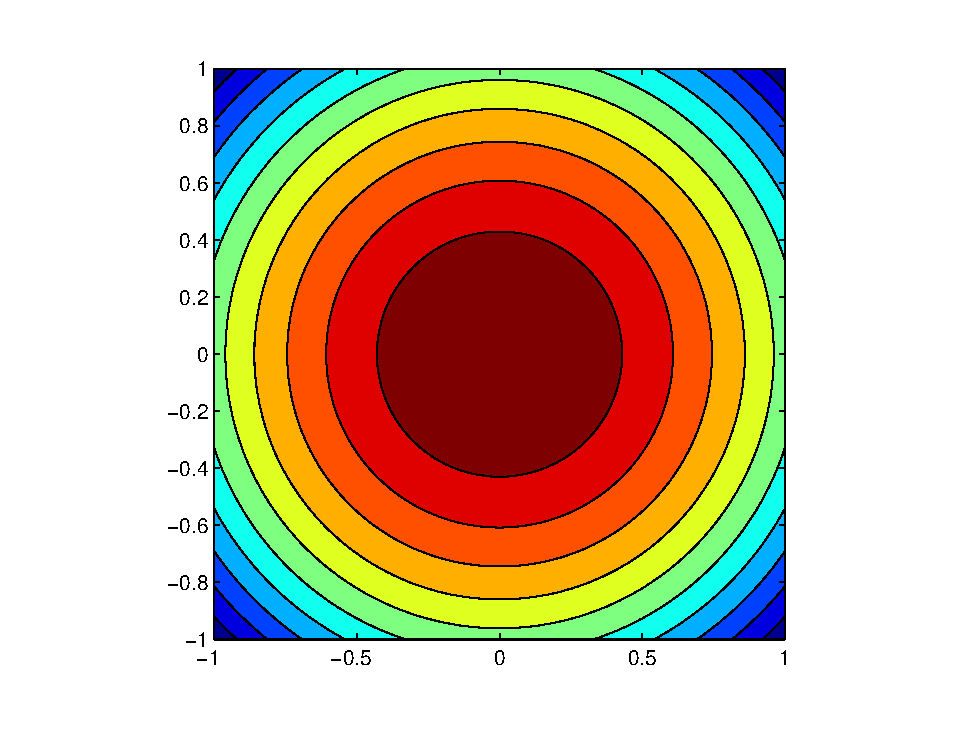
\includegraphics[width = 7cm]{images/courbes.eps}
%\caption{$1-k div_i$ for two characteristics and one object according to $r_{j1}$ and $r_{j2}$}
%\end{figure}

\subsection{Preprocessing : change variance and mean}
Since some judges might be more demanding in some characteristics than others, we propose to average all the ratings of a given judge in one characteristic and center them to $0$, and all the ratings should then be divided by their respective standard deviation. If there is only rating for one pair judge-characteristic then it should be set to zero. The normalized ratings should be used to compute the weights, then the original ratings are used with the weights computed.

According to the cases, we might want to choose to penalize some judges that give too high or too low ratings, or penalize some judge that have a high variance. As we will see, it is in fact not advised to divide the ratings by the standard deviation when dealing with dishonest judges. Indeed, they are likely to have a high varianc, and the normalizing is likely to rise their weight.

In some cases there might be ratings that are legal, but which are outside a certain scope relevant scope. If these should not be accounted for in the computing of the weights then they are of course to be removed.


\section{Properties of the method}
\subsection{Energy function for the method}
We know an energy function whose minimum corresponds to the fixed point of the iteration.\\
In order to deal with vector rather than tensors, we define the specific reputation (i.e. relative to a certain characteristic) column vector $ sr^k \in \mathbb{R}^{M\times 1}$ and the specific ratings matrix $sX^k \in \mathbb{R}^{N\times M}$
\begin{align*}
sr^k_{j} &= r_{jk} & sX^k_{ij} &= X_{ijk}
\end{align*}
Let's make the link between the energy function and the iteration. 
We can see that a fixed point $(r,w)$ of the proposed method satisfies $ w^{\star} = G(r^{\star})$ and is a solution of the following equation :
$$ (sr^k)^{\star} (\mathbf{1}^Tw^{\star}) = (sX^k)w^{\star} \:\: k = 1,..,K$$
or 
$$ (r_{jk})^{\star} \sum_{i=1}^N w_i^{\star} = \sum_{i=1} X_{ijk} w_i^{\star} \:\: j = 1,..,M \:\: k = 1,..,K$$
Which is simply a rewriting of the reputation function.


Hence we get by replacing appropriately that
\begin{align*}
((sr^k)^{\star} \mathbf{1}^T - (sX^k))\cdot G(r^{\star}) &= 0 & \forall k\in \{1,..,K\}
\end{align*}
This property is satisfied for any fixed point of the iteration. We will now define the energy function that we intend to minimize.
\begin{proposition}
The fixed points of the system are the stationary points of the energy function
\begin{align}
E(r) &=  \sum_{i=1}^n \int_0^{div_i(r)}g(u) \mathrm{d}u + c \label{eq:energy}
\end{align}
with $g(u) = 1 -ku$
\begin{proof}
Of course, the stationary points have zero gradient for each component.
$$
\frac{\partial E}{\partial r_{jk}} =  \sum_{i}\frac{\partial E}{\partial div_i} \cdot \frac{\partial div_i}{\partial r_{jk}} = 0
$$
The above formula is derived from the chain rule. We only have to replace the following expressions in the last equation
\begin{eqnarray*}
\frac{\partial div_i}{\partial r_{jk}} & = & \left[-\frac{2}{MK} (X_{i,j,:}-r_{j,:})\right]_{k} \\
\frac{\partial E}{\partial div_i} & = & g(div_i)\\
\end{eqnarray*}
Which yields
\begin{eqnarray*}
\frac{\partial E}{\partial r_{jk}} & = & \sum_{i}g(div_i) \cdot \left[-\frac{2}{MK} (X_{i,j,:}-r_{j,:})\right]_{k} 
\end{eqnarray*}
We can see that the condition $\frac{\partial E}{\partial r^{\star}_{jk}}=0 \:\: \forall j,k$ is equivalent to the fact that $(r^{\star},G(r^{\star}))$ is a stationary point of the iteration.
\end{proof}
\end{proposition}
\begin{proposition}
If the covariance matrix is the identity, one iteration in the system corresponds to a steepest descent step.
$r^{t+1} = r^t - \alpha_t \nabla_r E(r^t)$, with $\alpha^t = \frac{MK}{2 \sum_{i=1}^N w^t_i}$
\begin{proof}
We know that 
\begin{eqnarray*}
\frac{\partial E(r^t_{jk})}{\partial r^t_{jk}} & = & \frac{-2}{MK} \sum_{i=1}^N w_i (x_{ijk}-r^t_{jk})\\
& = & \frac{-2}{MK} (\sum_{i=1}^N w_i)(r^{t+1}_{jk}- r^t_{jk})
\end{eqnarray*}
Which proves the equality
\end{proof}
\end{proposition}
This energy function will prove useful when looking for convergence and uniqueness results.

\subsection{Interpretation}
We can also develop the expression of the energy function $E(r)$ and rewrite it as
$$ E(r) = \sum_{i=1}^N div_i - k \frac{div_i^2}{2} + c$$
If we take $c = \frac{2N}{k}$
Indeed, we then have $$ \sum_{i=1}^N div_i - k \frac{div_i^2}{2} + \frac{2N}{k}= -\frac{1}{2k}(1 - 2kdiv_i + div_i^2)$$
\\
The minimisation of the energy function is actually the minimisation of $  -\frac{1}{2k} w^Tw $.
So the method will actually find the reputation that will maximize the norm 2 of the weight vector. So it will favour a few large weights over more average weights. In other words, we maximize some kind of confidence but we want to be able to know which judges are to be trusted more.


\subsection{Uniqueness of the stationary point}

We can prove that the stationary point corresponding to our problem is unique under some assumptions on $k$.
We need $$k\in \mathcal{K} = \{k\in \mathcal{R}_{\geq 0} | 1 - k \begin{pmatrix} div_1 \\ div_2 \\ \vdots \\ div_n \end{pmatrix} >0 \: \forall r \in \mathcal{H} \}$$
where $\mathcal{H}$ is an hypercube. This ensures that the weights of the ratings are always positive. 

 Since $w$ has elements dependent in $r_{jk}^2$, the energy function is a polynomial of maximum order $4$ in each $r_{jk}$

There is a lemma in \cite{Cristo1} that goes as follows
\begin{lemma}
Let the function $E(r) : \mathbb{R}^n \rightarrow \mathbb{R} : E(r) = z $ be a fourth-order polynomial and let $\mathcal{H}$ be some hypercube in $\mathbb{R}^n$. If 
$$\lim_{||r||\rightarrow \infty} E(r) = - \infty $$
and the steepest descent direction on the boundary of $\mathcal{H}$ points strictly inside $\mathcal{H}$, then $E$ has a unique stationary point in $\mathcal{H}$ which is a minimum.
\label{eq:poly}
\end{lemma}
From which follows the following theorem
\begin{theorem}
If $k \in \mathcal{K}$, the system has a unique fixed point $r^{\star}$.\label{thm:uni}
\begin{proof}
The proof is similar to the uni-variable case. If any rating of a judge is the unique rating for an object and characteristic and is on the boundary of $\mathcal{H}$, we can exclude it from the iteration since we know that neither its corresponding reputation nor its participation in the weight of the judge will change over iterations. Hence we suppose that any object and characteristic receives at least two different votes. In that case, since we know that the votes belong to $\mathcal{H}$, we can say that the reputations at any point of the iteration will be in $int(\mathcal{H})$.
We also see that at any point on the boundary the next point will be in $int(\mathcal{H})$. Since the iteration corresponds to a steepest descent step for the energy function, we can say that the gradient on the boundary of $\mathcal{H}$ points inside $\mathcal{H}$. Since when $||r|| \rightarrow \infty$ the weights become infinitely negative, the Energy function satisfies the hypothesis of lemma \ref{eq:poly}. So there is a unique stationary point which is the fixed point of our system.
\end{proof}

\end{theorem}
We note that it is more likely in our multi-variate case to have some unique rating for some characteristic for an object. However, the given rating will determine the final reputation since the change in the weight of the judge won't change the reputation.
\subsection{Convergence}
By an argument similar to what is described in \cite{Cristo1}, we get the convergence result.
We will now prove the convergence of the method towards the unique minimizer of the energy function. In order to do that, we first need to prove a lemma :
\begin{lemma}
Let $c\in \mathbb{R}^{M \times K}$ a second order tensor, $M\in \mathbb{R}^{N\times M \times K}$ and $A\in \{0,1\}^{N\times M \times K}$ be third order tensors so that for $(i,j,k) \in \{1..N \times 1..M \times 1..K \}$ we have $M_{ijk} A_{ijk} = M_{ijk}$. ($M$ is the adjacency matrix of the votes).\\
Then we have 
$$\sum_{j=1}^M \sum_{k=1}^K (M_{ijk}-A_{ijk} c_{jk})^2 = \sum_{j=1}^M \sum_{k=1}^K M_{ijk}^2 - 2\sum_{j=1}^M \sum_{k=1}^K M_{ijk}c_{jk} + \sum_{j=1}^M \sum_{k=1}^K A_{ijk} c_{jk}^2$$
\begin{proof}
We simply use the hypothesis that $M_{ijk}A_{ijk} = M_{ijk}$ :
\begin{eqnarray*}
\sum_{j=1}^M \sum_{k=1}^K (M_{ijk}-A_{ijk} c_{jk})^2 & = & \sum_{j=1}^M \sum_{k=1}^K A_{ijk}(M_{ijk}-c_{jk})^2 \\
& = & \sum_{j=1}^M \sum_{k=1}^K A_{ijk} (M_{ijk}^2 - 2 M_{ijk}c_{jk} + c_{jk}^2)\\
& = & \sum_{j=1}^M \sum_{k=1}^K M_{ijk}^2 - 2\sum_{j=1}^M \sum_{k=1}^K M_{ijk}c_{jk} + \sum_{j=1}^M \sum_{k=1}^K A_{ijk} c_{jk}^2
\end{eqnarray*}
\end{proof}
\label{lemma:tens}
\end{lemma}

Now in order to show that the iteration does converge we will first show that the energy function decreases with the iterations.
\begin{lemma}
For the iteration described in equations \ref{eq:rep} and \ref{eq:w8} and the energy function defined as in equation \ref{eq:energy}, for an iteration $t\in \mathbb{N}$, we have 
$$(w^{t+1})^Tw^{t+1} \geq (w^t)^Tw^t$$
\begin{proof}
We will first express $w^{t+1}$ as a function of $w^t$.
Let $A$ be the adjacency tensor of the votes ($1$ if there is a vote, $0$ if not). Let $M = X - R^t$ with $X$ the tensor of the votes and $R^t_{ijk} = r^t_{jk}$ and let $c = r^{t+1}-r^{t}$. We can see that $A,M$ and $c$ all satisfy the hypothesis of lemma \ref{lemma:tens}.\\
Now let us remember that 
$$w_i^{t+1} = 1 - k \frac{1}{MK} \sum_{j=1}^M \sum_{k=1}^K A_{ijk}(X_{ijk}-r_{jk})^2$$
which can be replaced by
\begin{eqnarray*}
w^{t+1} & = & 1 - \frac{k}{MK} \sum_{j=1}^M \sum_{k=1}^K  (M_{ijk} - A_{ijk}c_{jk})^2\\
& = & 1- \frac{k}{MK}\left[ \sum_{j=1}^M \sum_{k=1}^K (M_{ijk})^2 - 2 \sum_{j=1}^M \sum_{k=1}^K c_{jk}M_{ijk} + \sum_{j=1}^M \sum_{k=1}^K  c_{jk}^2 \right]\\
& = & 1 - \frac{k}{MK}\left[ \sum_{j=1}^M \sum_{k=1}^K (X_{ijk}-r_{jk}^t)^2  - 2 \sum_{j=1}^M \sum_{k=1}^K (r^{t+1}_{jk}-r^t_{jk})(X_{ijk}-r^t_{jk}) \right.\\
& & \left. + \sum_{j=1}^M \sum_{k=1}^K  (r^{t+1}_{jk} - r^t_{jk})^2 \right]\\
& = & w^t + \frac{k}{MK} q
\end{eqnarray*}
with $q = 2 \sum_{j=1}^M \sum_{k=1}^K (r^{t+1}_{jk}-r^t_{jk})(X_{ijk}-r^t_{jk}) - \sum_{j=1}^M \sum_{k=1}^K  (r^{t+1}_{jk} - r^t_{jk})^2 $
\end{proof}
\end{lemma}

As a consequence, we have
\begin{eqnarray*}
(w^{t+1})^Tw^{t+1} & = & (w^t)^Tw^t + \frac{k^2}{M^2K^2} q^Tq + 2 \frac{k}{MK} q^T w^t
\end{eqnarray*}
We need to show that $q^Tw^t \geq 0$.

\begin{eqnarray*}
q^Tw^t & = & 2 \sum_{i=1}^N w^t_i (\sum_{j=1}^M \sum_{k=1}^K (r^{t+1}_{jk}-r^t_{jk})(X_{ijk}-r^t_{jk}) - \sum_{i=1}^N w^t_i \sum_{j=1}^M \sum_{k=1}^K  (r^{t+1}_{jk} - r^t_{jk})^2)\\
& = & \sum_{j=1}^M \sum_{k=1}^K (r^{t+1}_{jk}-r^t_{jk}) \sum_{i=1}^N w^t_i (X_{ijk}-r_{jk}^t)- (\sum_{i=1}^N w^t_i) \sum_{j=1}^M \sum_{k=1}^K  (r^{t+1}_{jk} - r^t_{jk})^2)\\
& = & (\sum_{i=1}^N w^t_i) \sum_{j=1}^M \sum_{k=1}^K  (r^{t+1}_{jk} - r^t_{jk})^2)\\
& \geq & 0
\end{eqnarray*}
We used here the fact that $\sum_{i=1}^N w^t_i (X_{ijk}-r_{jk}^t) = (\sum_{i=1}^N w^t_i) \sum_{j=1}^M \sum_{k=1}^K  (r^{t+1}_{jk} - r^t_{jk})^2$ by definition of the reputations.
We also have 
$$E(r^{t+1})- E(r^t) \leq \frac{-\delta}{MK} \sum_{j=1}^M \sum_{k=1}^K (r^{t+1}_{jk} - r^t_{jk})^2$$
We know that the sequence of the $r^t$ will not go out of $int(\mathcal{H})$.
Since $E$ is lower bounded on $int(\mathcal{H})$ and that $E$ decreases at each iteration, the sequence will converge. We know also from \ref{thm:uni} that we have converged to the unique minimum of $E$ in $int(\mathcal{H})$


\subsection{Sparsity}

This section extends some previous results to the case where the rating matrix is sparse, i.e. when an object is not evaluated by all judges and/or not in all characteristics. In many real-life example we need to deal with the data that is structurally sparse. If we take the example of teachers who rate the students on various courses that are relevant only to some characteristics, it is clear that teachers will rate only their own course and therefore not give a rating to all characteristics. We can hardly find a set of judges, objects and characteristics with a vote for all possible values.\\

A vote absence for object $i$ from judge $j$ on characteristic $k$ will imply that the entry $(i, j, k)$ of the tensor $X$ is equal to zero (The reverse is not true). That is why we introduce the adjacency tensor $A \in \mathbb{R}^{N \times M \times K}$, if $A_{ijk} = 0$, then $X_{ijk}$ = 0. These entries must not be considered as votes but instead as missing values. Therefore the previous equations presented in matrix form require some modifications that will include the adjacency tensor $A$.


\subsubsection{Iterative filtering systems}
 The column vector $d_k^{ij}$ defined in section \ref{section:sub:iteration} becomes
 
\[
    d^{ij}_k = X_{ijk} - A_{ijk}   \cdot r_{jk}
\]

This latest vector can be seen as the distance of the ratings of the judge $i$ for object $j$ from the reputation of the object $j$ on evaluated characteristics.

\subsubsection{Quadratic iterative filtering systems}

The reputation matrix $F(w, X)$ is now given by

\[
    F_{jk}(w, X) = \frac{\sum_i x_{ijk}w_i}{\sum_i A_{ijk}w_i}
\]

It is simply the sum of the characteristics ratings weighted by the weights of all the judges on this characteristics. Let us remark that the denominator must be strictly positive. This means that every characteristics is evaluated by at least one judge with non-zero weight !\\

\[
    div_i = \frac{1}{m_i} \sum_{j=1}^{N} (d^{ij})^TC^{-1}(d^{ij})
\]

\[
    G_i(X, r, C) = 1 - k \cdot div_i
\]

with
\[
    m_i = \sum_{j=1}^{N} \sum_{k=1}^{K} A_{ijk} \qquad \text{ and } \qquad k = \frac{1}{(\log(2\pi)\det(C)}
\]

All previous proofs still apply.


\section{Extensions and particular cases}
\subsection{Total score and weighting of characteristics}
At some point it is often expected from a reputation system to provide a final score for an object. This score can be weighted according to some new parameters $p_k$, each relative to a characteristic.
The first option to account for this is to simply compute the reputations for each characteristic and then perform a weighted sum.
$$ s_j = \sum_{k=1}^K p_k r_{jk} $$
A second option would be to include directly the weighting of the votes inside the calculation of the reputations. We can do this by first multiplying the votes $X_{ijk}$ by the weighting $p_k$. 
$$X'_{ijk} = p_k X_{ijk}$$
This way we will make the ratings in the characteristics with higher ratings more important. It means that an incoherent rating in one of those important ratings will be very penalizing for a judge. This variant can be chosen if we do want to implement that.
The final rating will be calculated as the sum of the resulting $r'_{jk}$s
$$ s_j = \sum_{k=1}^K r'_{jk}$$

\subsection{Interdependence of some characteristics}
%Suppose that one judge is the only one to give some object a rating. If this is the case for all the objects, all the weights will be equal to $1$.\\
%A way to avoid this is by introducing some dependence between the characteristics of the objects.\\
%$$div_i = \sum_{j=1}^N \sum_{k=1}^K A_{ijk} \sum_{k2=1}^K l_{k,k2} (X_{ijk}-r_{jk2})^2$$
%Where $l_{k,k2}$ represents a dependence between two characteristics. This way, if there is only one rating in one characteristic, the weight of the judge who gave this rating will be influenced by the other reputations.
We might want to include the dependency of one characteristic according to another.

Let $C$ be a covariance matrix between characteristics. This means that the rating in two characteristics of an object can be linked in some way. 
We keep the usual computation of the reputations as the weighted sum of the ratings as in equation \ref{eq:rep}. The weights would need to be modified. We keep equation \ref{eq:w8} but we modify the definition of $div_i$.
$$div_i =  \frac{1}{MK}\sum_{j} (d^{ij})^T C^{-1} (d^{ij})$$
Introducing covariances would mean that we "allow" some judge (in the sense that we don't reduce its weight too much) to be partial and give incoherent marks if it is consistent with the covariances.\\
In the case of a diagonal matrix, the result of convergence can be easily reproduced, but we did not find a proof for the general case. This extension was not implemented.


\subsection{Several judges agree on one rating}
If several judges give a common rating to one object, we can assume that the rating given is the result of the mean of the ratings that each judge would have given separately. At first we simply put the value of the rating in each of the rating of the judges. We can see that this rating will be given more weight since it is given by several judges. So we can assume that the weights of the judges will increase compared to the case where a judge is alone to give a rating. 

\section{Influence of $k$}
When we applied this method, we are confronted with the choice of the parameter value $k$. In situations where we expect some judges to be unreliable, we might want to choose $k$ as high as possible in order to differentiate the reliable judges from the unreliable.

That is why an alternative to a constant $k$ is proposed in \cite{Cristo1}. Instead of using a constant $k$, we use a sequence $k^t$. The sequence is such that at each iteration the weights are non-negative.
$$ k^t : \min_i w_i^t = 0$$
If the sequence converges, so does the iterative filtering, and we are left with a value of $k$ for which the weights are always positive.
Although we didn't find any proof of the convergence of the sequence, we know that it is bounded below by zero and it is bounded above if there are at least 2 ratings for one characteristic of an object.	The sequence converged for every data set we tried. In general it is better to choose $k^t$ so that the smallest weight is slightly above zero to avoid numerical problems.
But, we notice that the more cheaters there are, the smaller the highest possible $k$. As a result, there can be cheaters with very incoherent ratings that will reduce the maximum $k$, and hence will shield other more subtle cheaters weights from being heavily reduced.
This is obviously a shortcoming of the model, but other methods such as the outlier method are also subject to such problems.

\section{Cheating}
How does a cheater determine which value to give his ratings in order to maximize a final rating? 
\subsection{Intuitive cheating}

The cheater who would want to increase the reputation of one object in one characteristic would be tempted to simply rise his rating for this object and characteristic. Although this is not a guarantee of success, we will show that we can easily find an half hyperspace in which the new reputation will be situated.\\

Let's take as usual a tensor of ratings $X$ and a matrix of reputations $r^{\star}$ that corresponds to the minimum of the energy function. Now we assume that judge $t$ who we will call the cheater will want to change the global reputation and changes his ratings. So we can suppose that he can only change the rating $X_{tjk}$. 

So the modified tensor $X'$ is equal in all ratings to $X$, except in $(t,j,k)$ for all $j,k$ so that $A_{tjk}=1$. The resulting modified reputation matrix is $r'$. The new energy function relative to the modified ratings is $E'(r')$.
\begin{lemma}
The vector of reputation for the initial ratings $r^{\star}$ is actually the minimum of the new energy function subject to the constraint that $\langle (r'-r^{\star}),\nabla_{r'} E'(r')\rangle = 0$. In other words, 

\begin{align*} 
 E'(r^{\star}) & = &  \min_{r'\in \mathcal{H}} & E'(r')& \\
& & s.t.  \:\:  & \langle r'-r^{\star},\nabla_{r'} E'(r^{\star}) \rangle =0
\end{align*}

\begin{proof}
The Lagrangian of the problem can be written as
$$\mathcal{L}(r') = E'(r') - \lambda (\langle r' - r^{\star},\nabla_{r'} E'(r^{\star}) \rangle )$$

Using lemma \ref{eq:poly}, there cannot be maximas or saddle points in $\mathcal{H}$ and the minimum is unique in this domain. Hence there must be only one point in the restriction of $E'$ that satisfies the KKT conditions, and it will be the minimum.\\
They can be written as follows :
\begin{align*}
\nabla_{r'} E'(r') - \lambda \nabla_{r'} E'(r^{\star}) & = & 0\\
\langle r'-r^{\star},\nabla_{r'} E'(r^{\star}) \rangle & = & 0
\end{align*}
We can see that these conditions are satisfied for $r' = r^{\star}$ and $\lambda = 1$. So $r^{\star}$ is the minimum for $<r'-r^{\star},\nabla_{r'} E'(r^{\star})>=0$
\end{proof}
\end{lemma}


\begin{proposition}
The change of the ratings $X_{tjk}$ in new ratings $X'_{tjk}$ for some judge $t$ for all $j,k$ automatically leads to a new reputation tensor $r'^{\star}$ which satisfies 
$$ \langle c, r'^{\star} - r^{\star} \rangle \geq 0$$
with $c_{jk} = ( w'_t(r^{\star})- w_t) (X'_{tjk}-r^{\star}_{jk}) + w_t(X'_{tjk}-X_{tjk}) $.
\label{pr:hyperp}
\begin{proof}
Let us first look at the gradient of the energy function.
$$\frac{\partial E'(r')}{r'_{jk}} = \sum_{i=1}^N w_i(r') (-2 (X'{ijk}-r'_{jk}))$$

Let $w'(r')$ be the vector of new weights for the judges, computed from the new ratings ($X'$) and the reputations $r'$.
If $r' = r^{\star}$, we know that since the ratings of all the normal judges haven't changed, their weights are also the same , thus $w'_i(r^{\star}) = w_i^{\star}$ for $i \neq t$. We also know that since $r^{\star}$ is the minimum of $E$, we have 
$$ \frac{\partial E(r^{\star})}{r_{jk}} = \sum_{i=1}^N w_i (-2 (X{ijk}-r^{\star}_{jk})) = 0$$
and 
$$ \frac{\partial E'(r^{\star})}{r'_{jk}} = \frac{\partial E(r^{\star})}{r_{jk}}+2w_t(r^{\star})(X_{tjk}-r^{\star}_{jk})-2 w'_t(r^{\star}) (X'_{tjk}-r^{\star}_{jk}) $$
Hence we can write
$$ \frac{\partial E'(r^{\star})}{r'_{jk}} = -2 \left[ ( w'_t(r^{\star})- w_t) (X'_{tjk}-r^{\star}_{jk}) + w_t(X'_{tjk}-X_{tjk}) \right]$$

When we compute the new reputation, we can start the iteration from the former $r^{\star}$. So we will use a sequence of $(r')^t$, $(w')^t$ which will converge towards $r'^{\star}$ and $(w')^{\star}$.
We take $(r')^0 = r^{\star}$ and $(w')^0 = G(X',r^{\star})$. We know that the next iteration will be 
$$ (r')^1 = (r')^0 - \alpha \nabla_{r'}E((r')^0)$$
Since $\alpha$ is chosen greater than zero, we can see that $\langle (r')^1 - (r')^0, \nabla_{r'}E((r')^0) \rangle$ is less or equal to zero.
Hence 
\begin{eqnarray*}
\langle (r')^1 - r^{\star}, \nabla_{r'}E(r^{\star})\rangle & \leq & 0\\
\langle (r')^1 - r^{\star}, -2 c\rangle & \leq & 0\\
\langle (r')^1 - r^{\star}, c\rangle & \geq & 0
\end{eqnarray*}
Here we needed to assume again that the weights are non-negative for the iteration.

At this point, we know that $\langle (r')^1 - r^{\star}, c\rangle  \geq  0$.
So now let's suppose that $\langle(r')^{\star} - r^{\star}, c\rangle  <  0$. Hence there would be a point $\tilde{r}$ sitting on the line between $(r')^{\star}$ and $(r')^1$ which would satisfy $\langle \tilde{r}- r^{\star}, c\rangle = 0 $. and Since $E'$ diminishes at every iteration it would imply that $E'(r'^{\star}) \leq E'((r')^1) \leq E'(\tilde{r}) $. That would imply that there is a local maximum on the restriction of $E'$ on the line between $(r')^{\star}$ and $(r')^1$, but that is impossible from lemma \ref{eq:poly}.
\end{proof}

\end{proposition}

The result of the previous theorem is illustrated in figure \ref{hyperp}, in which we can see in green the admissible region of the new reputations. It is the intersection of the convex hull of the rating of the judges and the half space described by the hyperplane described in proposition \ref{pr:hyperp}. We see that increasing a rating does not necessarily increase the reputation. Here indeed the weight of judge $t$, will diminish, which will lead to the reputation receding from the rating of judge $t$.
\begin{figure}[h!]
\centering
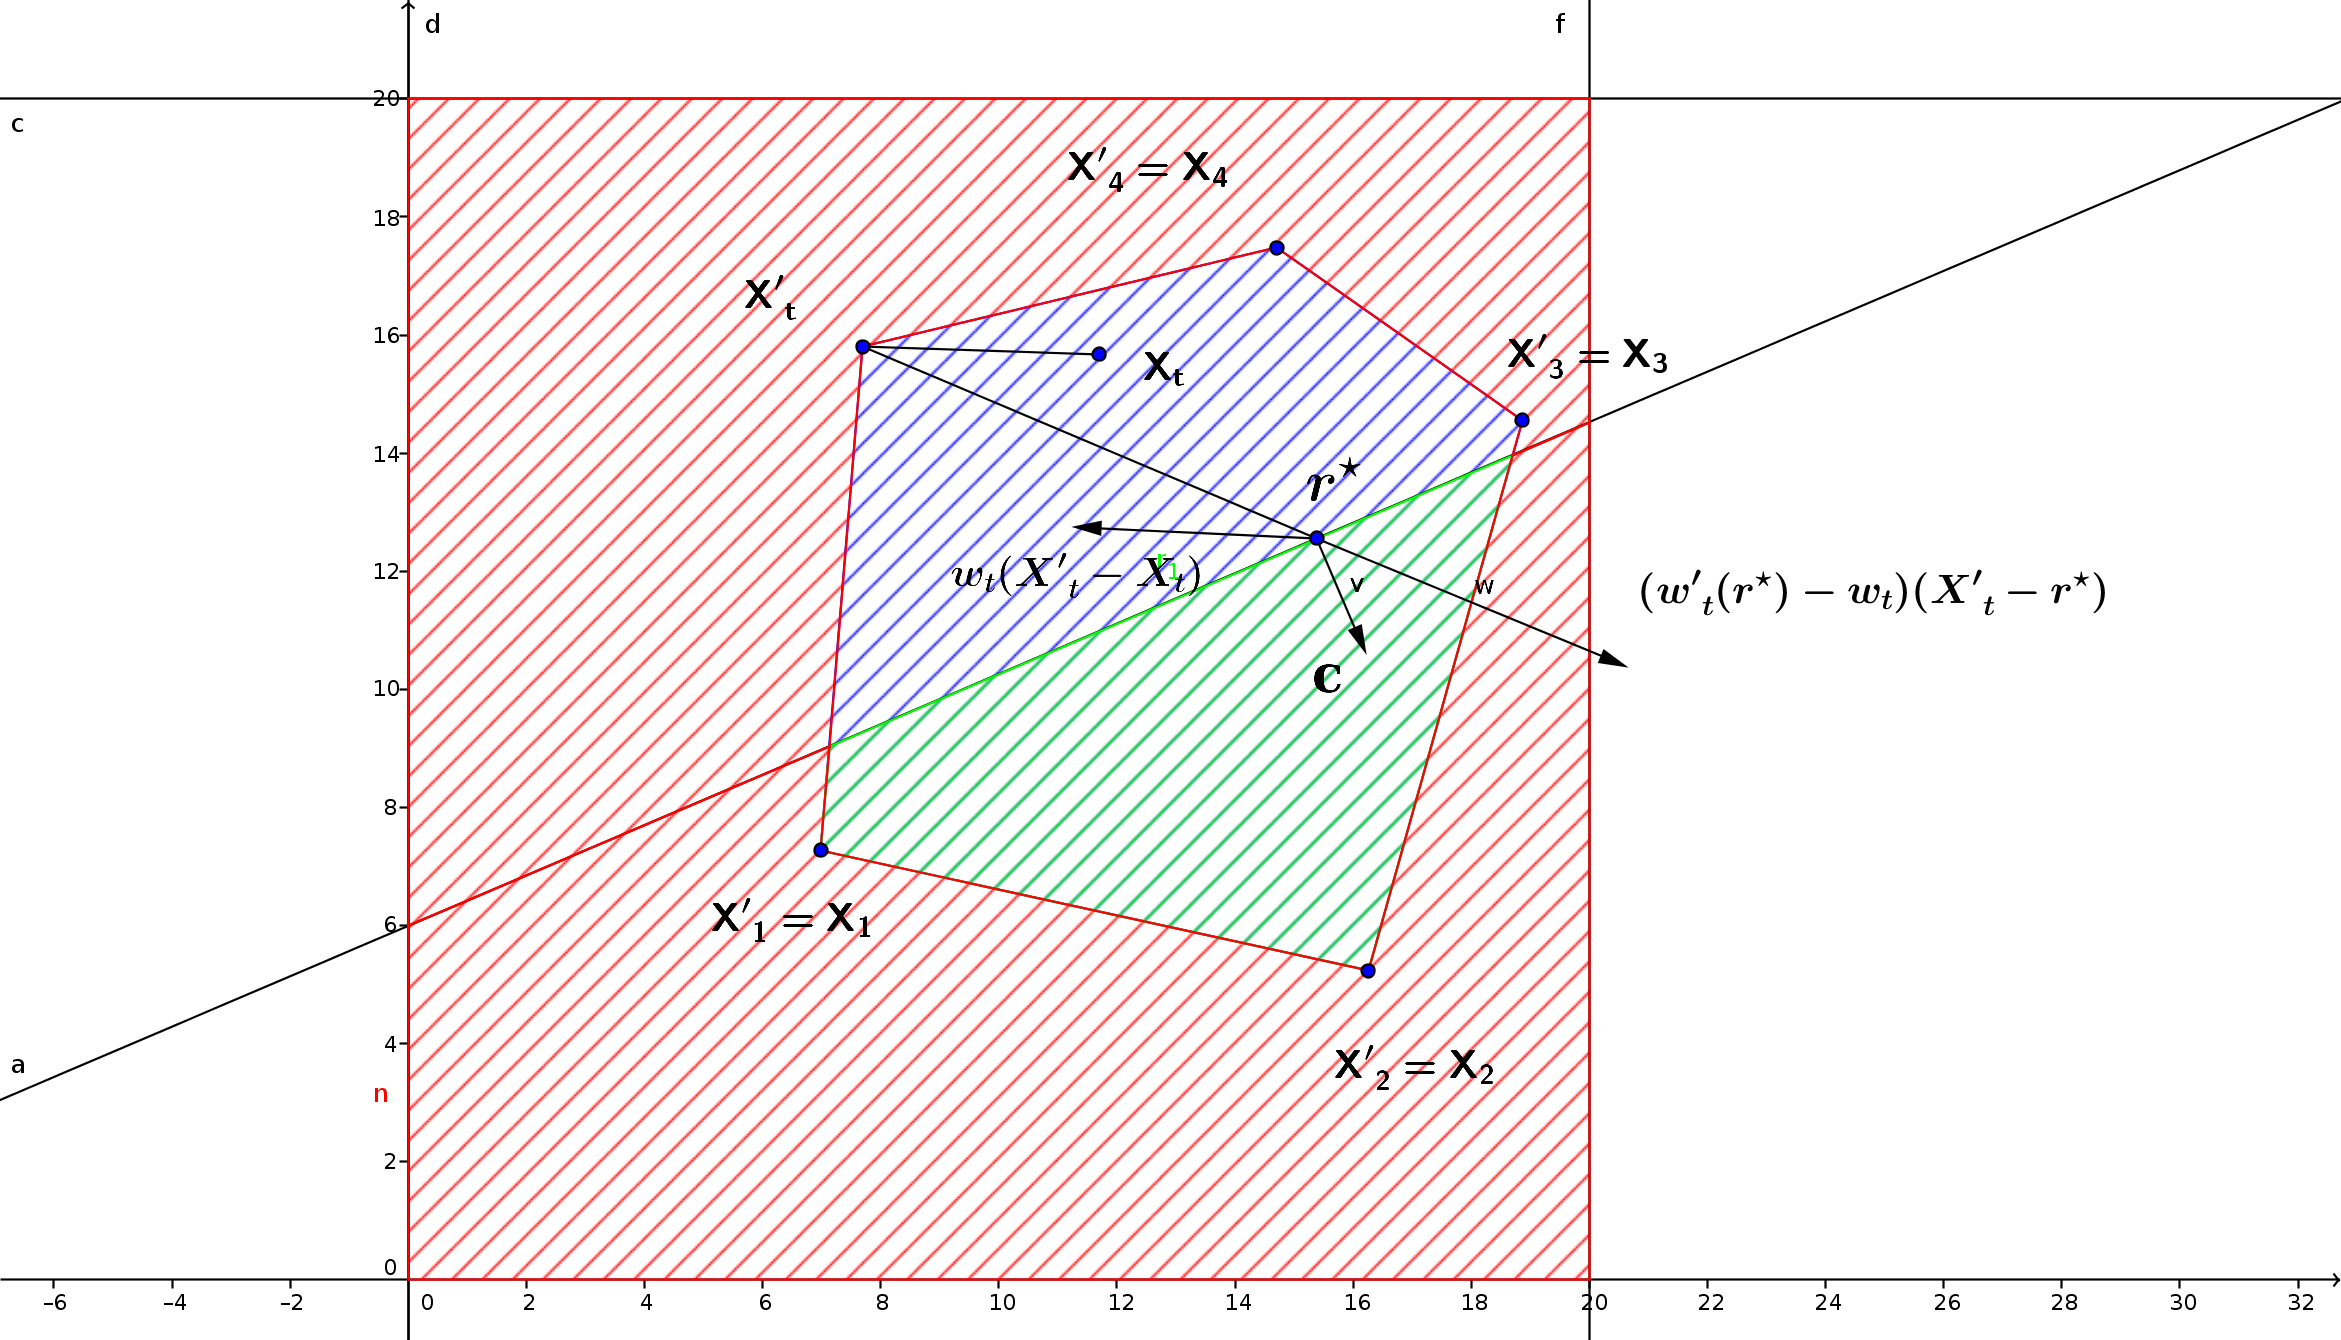
\includegraphics[width = 12cm]{geogebra/Hyperplane.png}
\caption{\label{hyperp}Illustration of the proposition}
\end{figure}
\FloatBarrier
\subsection{Monotonicity}
We suppose that when a judge already has many votes, his weight will diminish very slowly when he recedes from the reputation of the object.\\
The question we need to answer is whether the highest rating we can give will result in the maximum reputation that we can get. In other words, we are looking for cases where the final reputation will not evolve monotonously according to a certain rating. If there were no such case, the optimal behaviour of the cheater would be trivial since he only needs to put the maximum rating to some characteristic of some object in order to maximize the corresponding reputation.\\

The figure (\ref{fig:howto}) shows a case where we have two teams, and three different ways to evaluated them (characteristics). The goal of the cheater is helping the first team to win. That is why we only observe the score obtained by the first team called "Advantaged Team". Notice that the cheater knows only his notes! We present three ways of computing the mean.
\begin{enumerate}
    \item The basic mean that is a linear function. It is obvious that the cheater must give the maximum note to the advantaged team.
    \item The "outlier method" or truncated mean which consists to discard the lowest and the highest scores and calculate the mean value of the remaining scores. In this case we have a piecewise linear function. It is also obvious that the cheater must give the maximum note to the advantaged team, although the maximum reputation is lower.
    \item The iterative method. In this case we see that if the cheater wants the note of the favoured team to be maximum, then it should not give them the maximum score! Here, the cheater has put a score of 0 to the disadvantaged team. If the cheater had put a note of 10 to the second team, the function would have been monotonous.
\end{enumerate}
We can conclude that the iterative method does not allow the cheater to know what to do in advance. It is also possible to show a similar graph if we want to disadvantage a team.

\begin{figure}[h!]
\centering
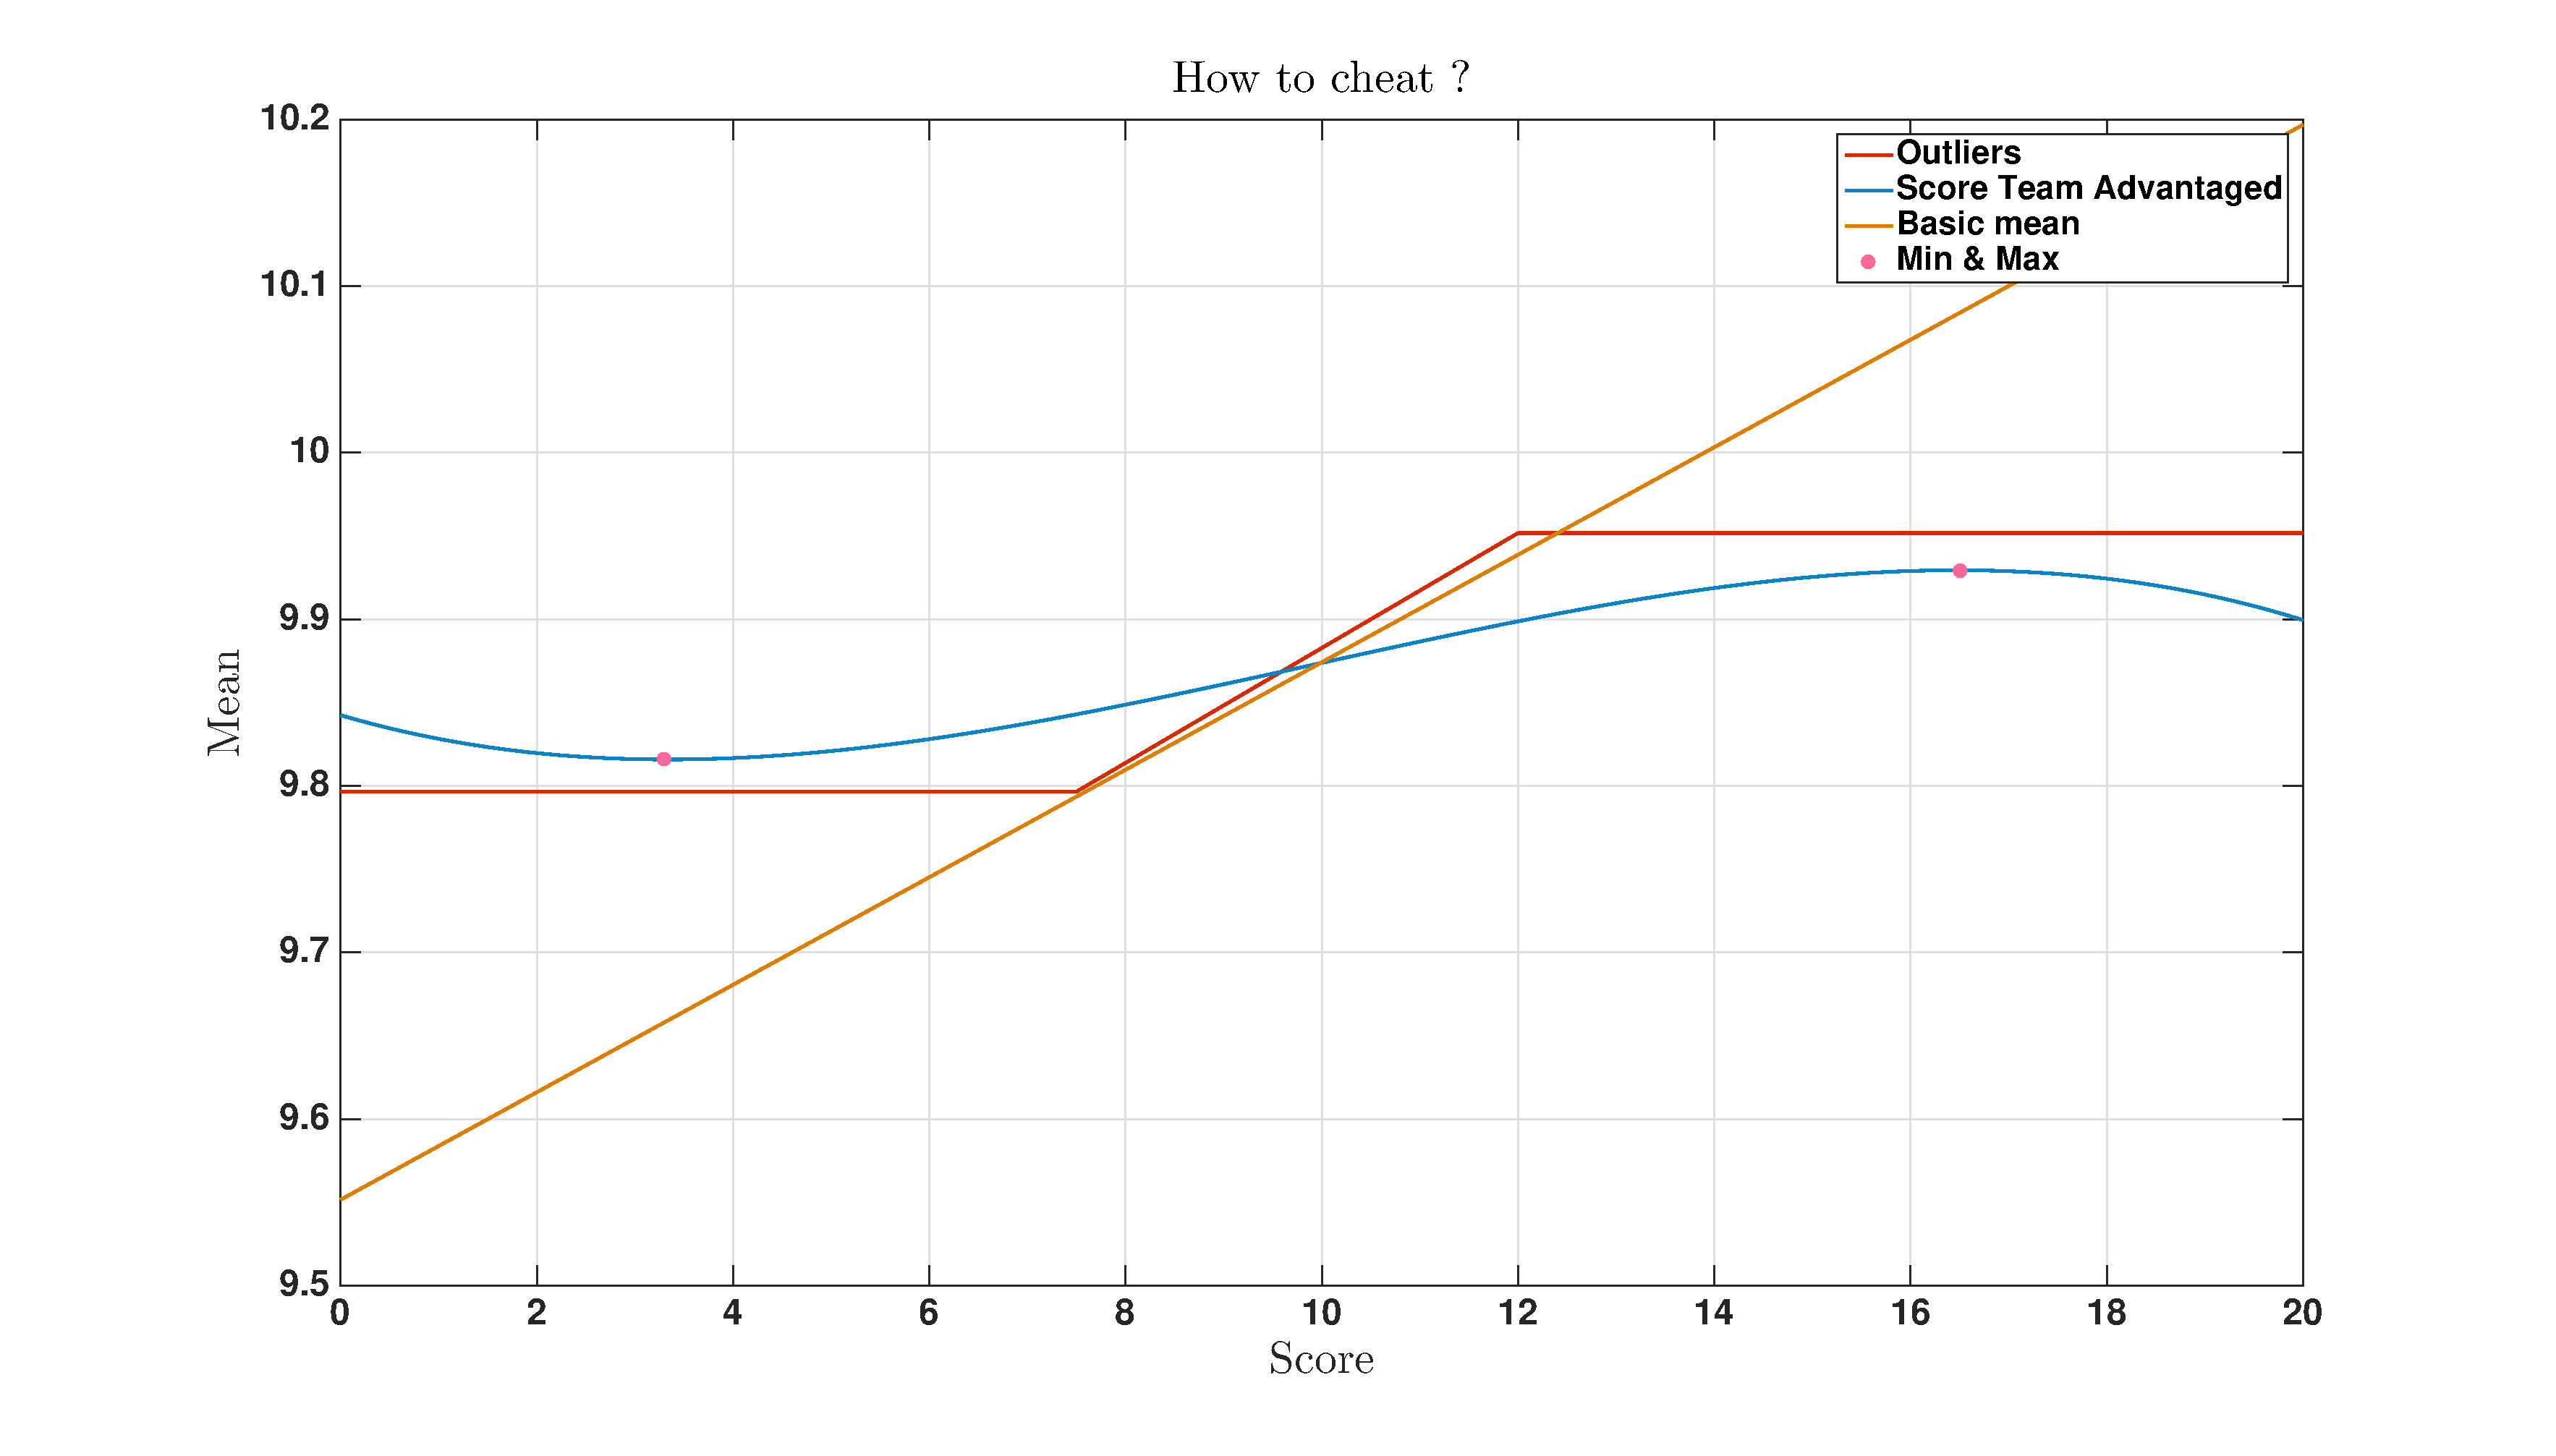
\includegraphics[width = 0.75\textwidth]{cheaters/howto.eps}
\caption{Evolution of the assessment of a team depending on the choice of cheater}
\label{fig:howto}
\end{figure}

The figure (\ref{fig:howto_weight}) show the evolution of the cheater's weight associated to the figure (\ref{fig:howto}).

\begin{figure}[h!]
\centering
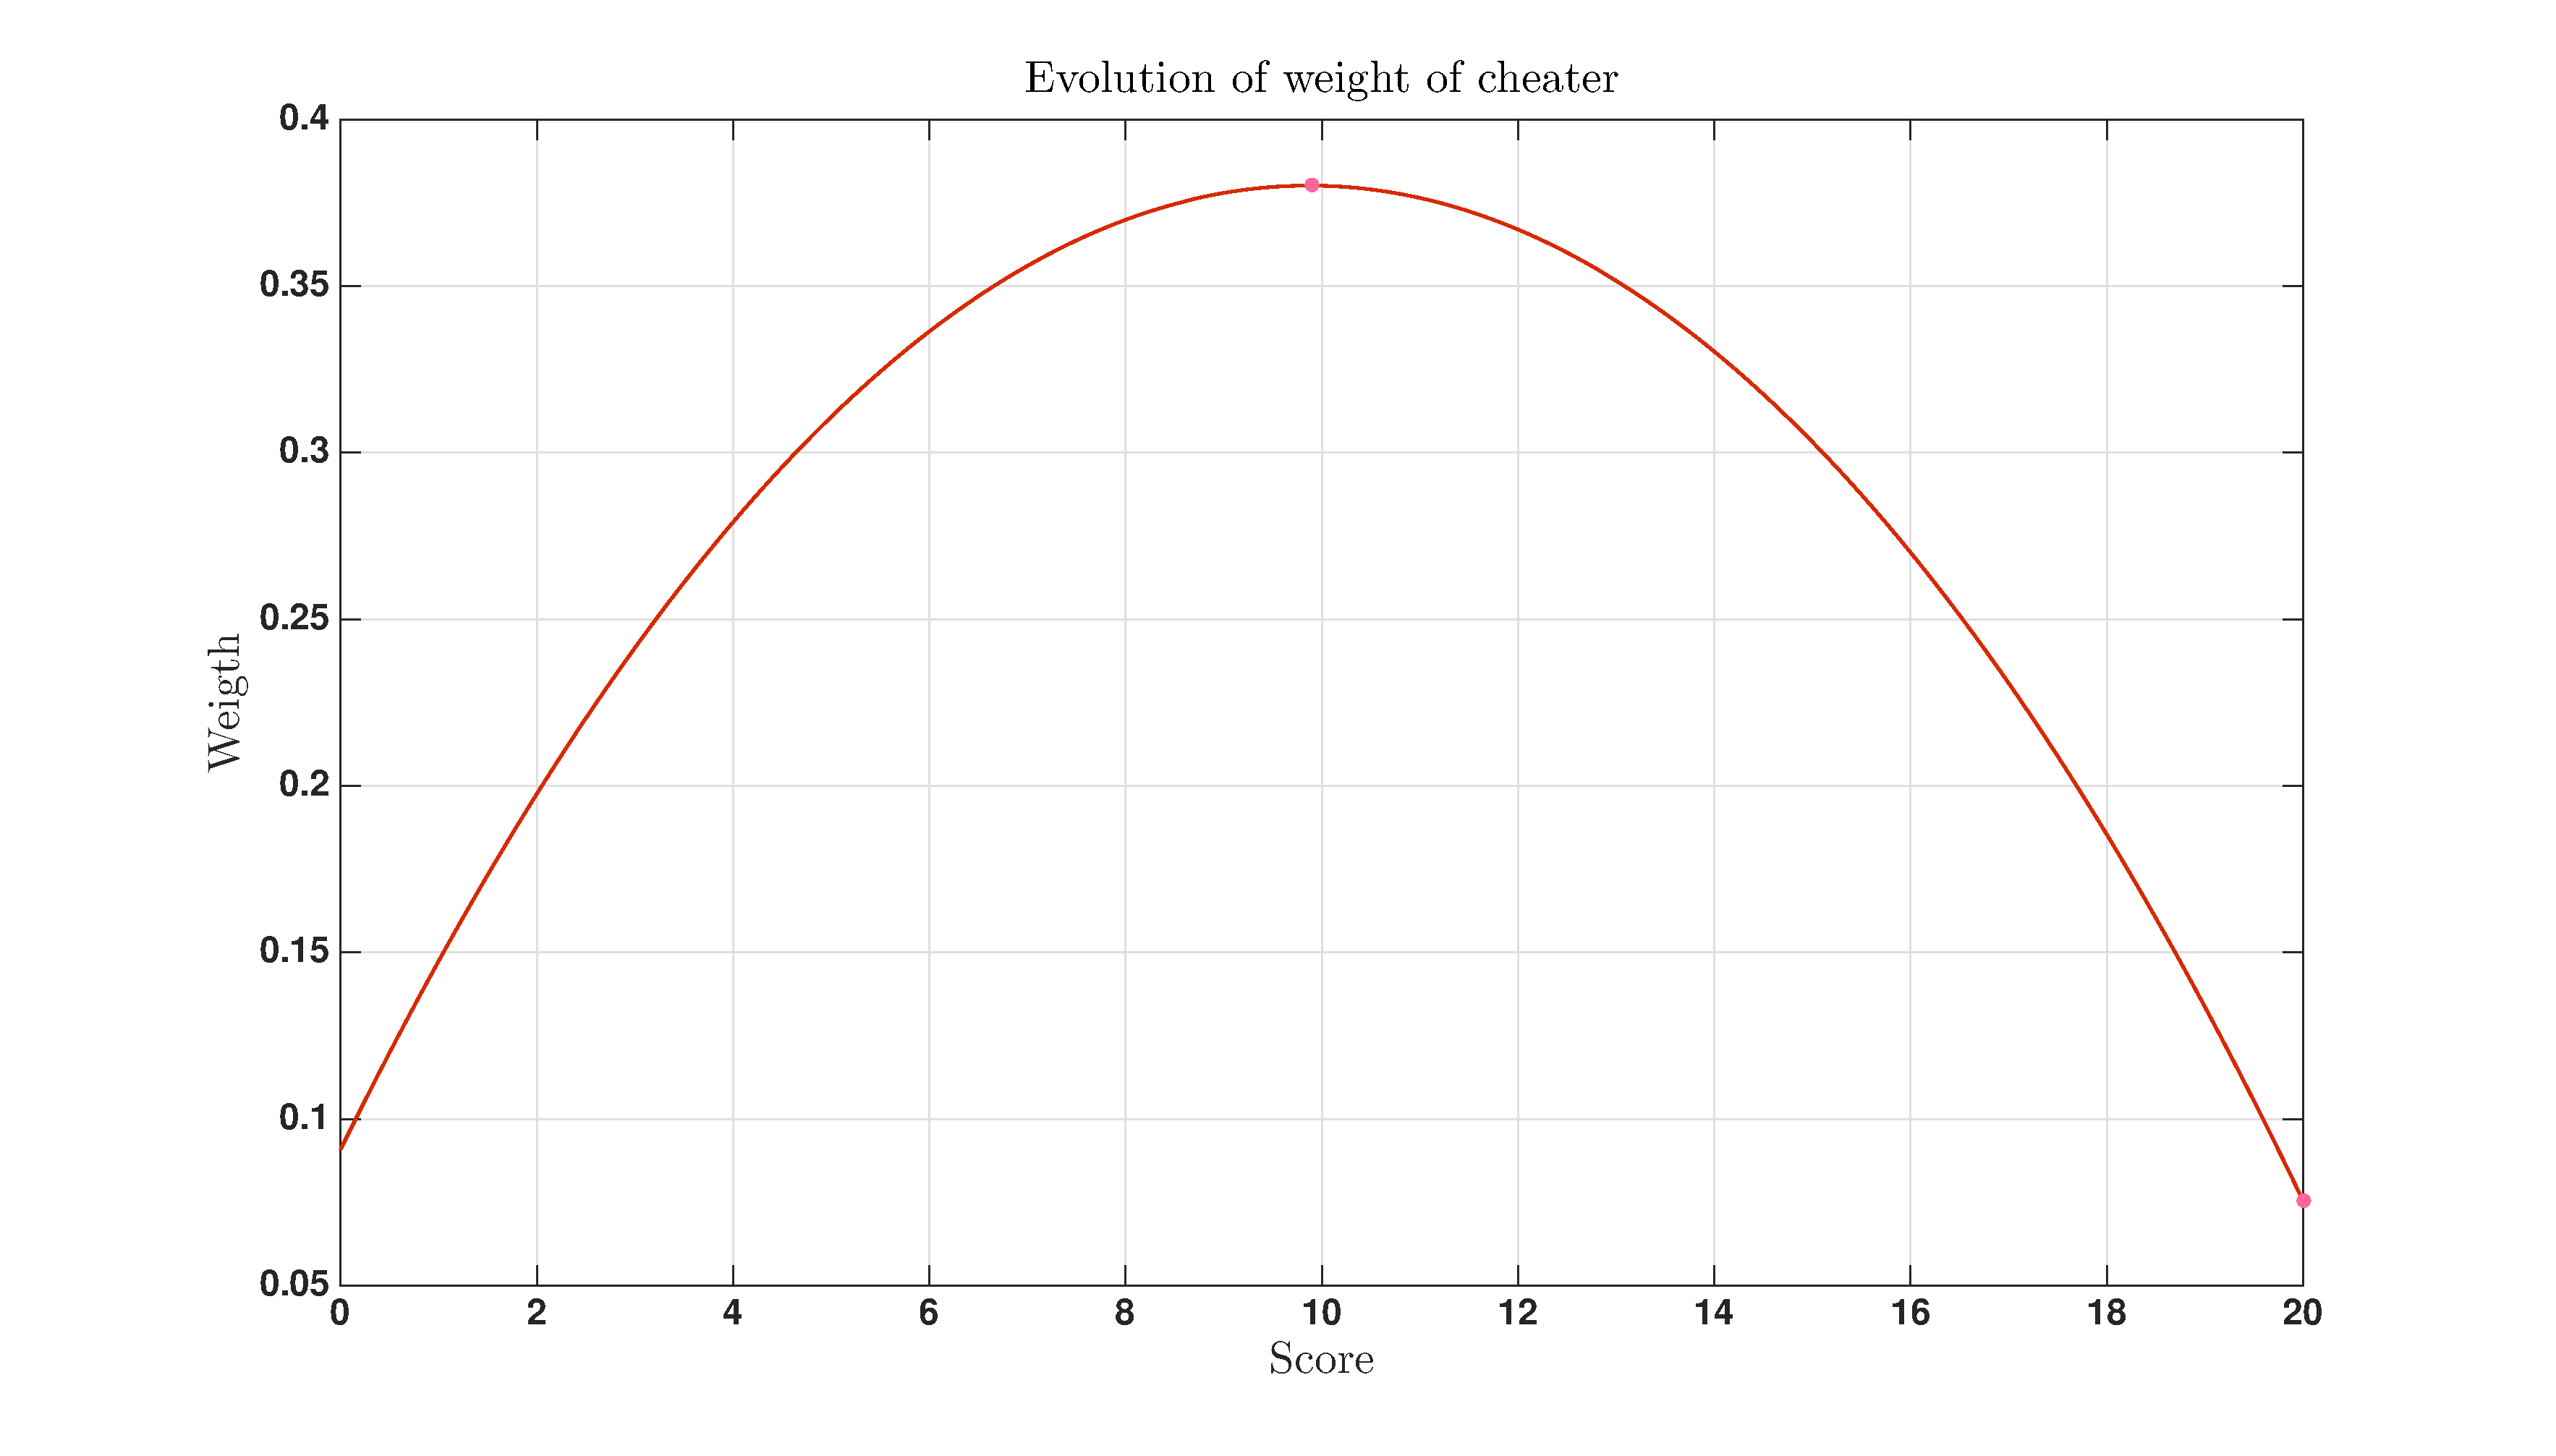
\includegraphics[width = 0.75\textwidth]{cheaters/evolution_cheater_weight.eps}
\caption{Evolution of cheater's weight}
\label{fig:howto_weight}
\end{figure}

\section{Application to MAP scores}
We were given the scores of the students in the applied mathematics program from 2011 to 2014. Here we did not expect to have significant results on the reliability of some teachers, since we can always choose the value of $k$ so that the least reliable judge has a weight zero. Instead, we discuss the preprocessing to apply to this data and the influence of several factors such as the number of rating of a judge with his weight.


\FloatBarrier
\subsection*{Influence of mean rating}
First, let us look at the average (figure \ref{mean1}) and variance (figure \ref{var1}) of ratings for each teacher in each characteristic.
\begin{figure}[h!]
\centering
\begin{subfigure}[b]{0.49\textwidth}
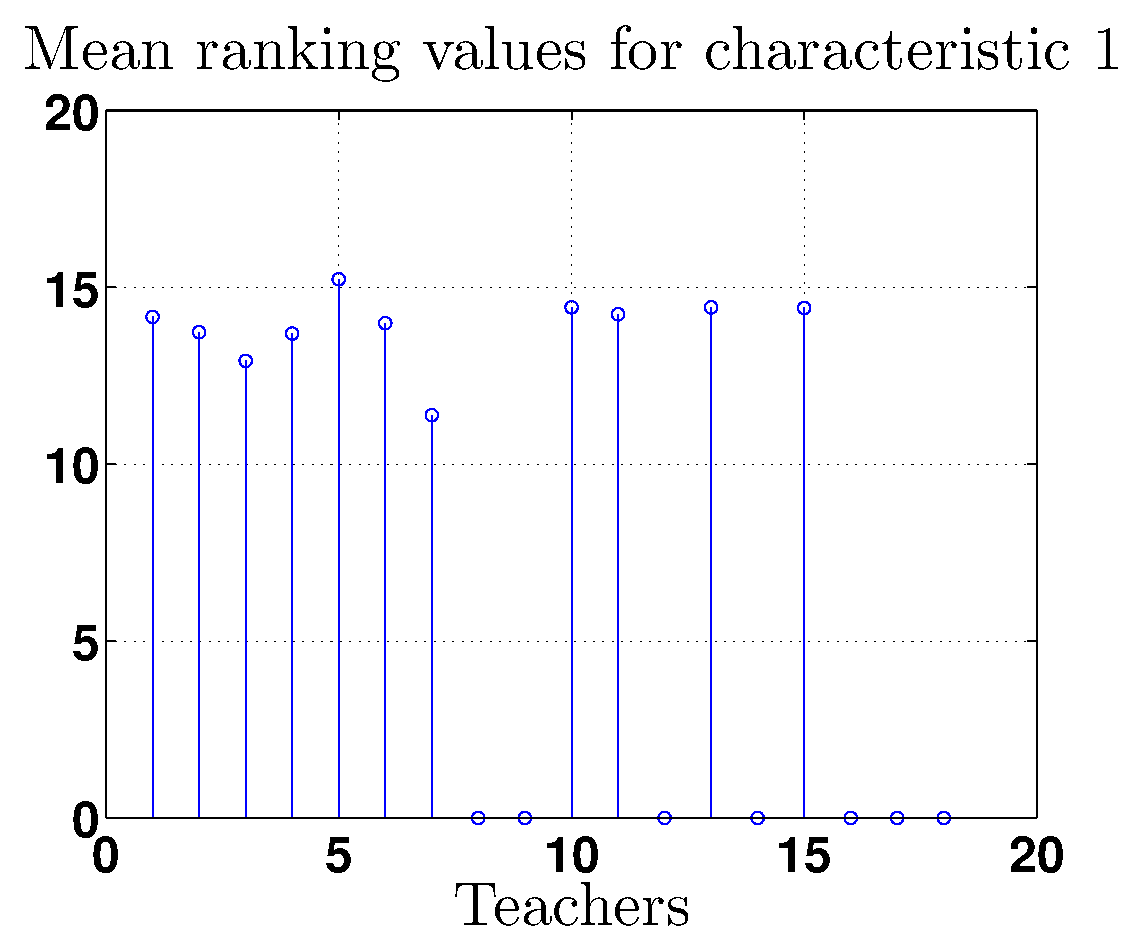
\includegraphics[width = 5cm]{noPreprocess/meanTeachersC1.eps}
\end{subfigure}
\begin{subfigure}[b]{0.49\textwidth}
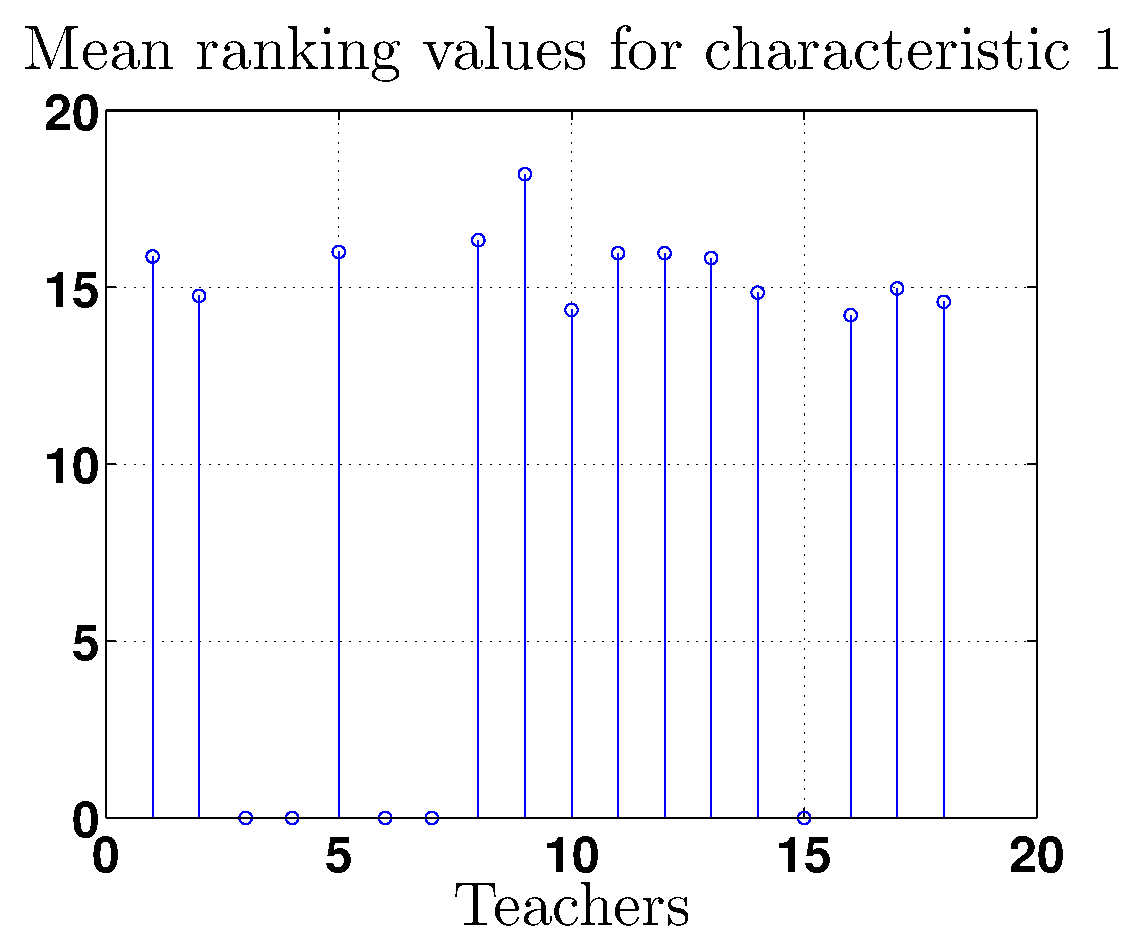
\includegraphics[width = 5cm]{noPreprocess/meanTeachersC2.eps}
\end{subfigure}
\caption{Mean ratings of teachers for mandatory and optional courses\label{mean1}}
\end{figure}
\begin{figure}[h!]
\centering
\begin{subfigure}[b]{0.49\textwidth}
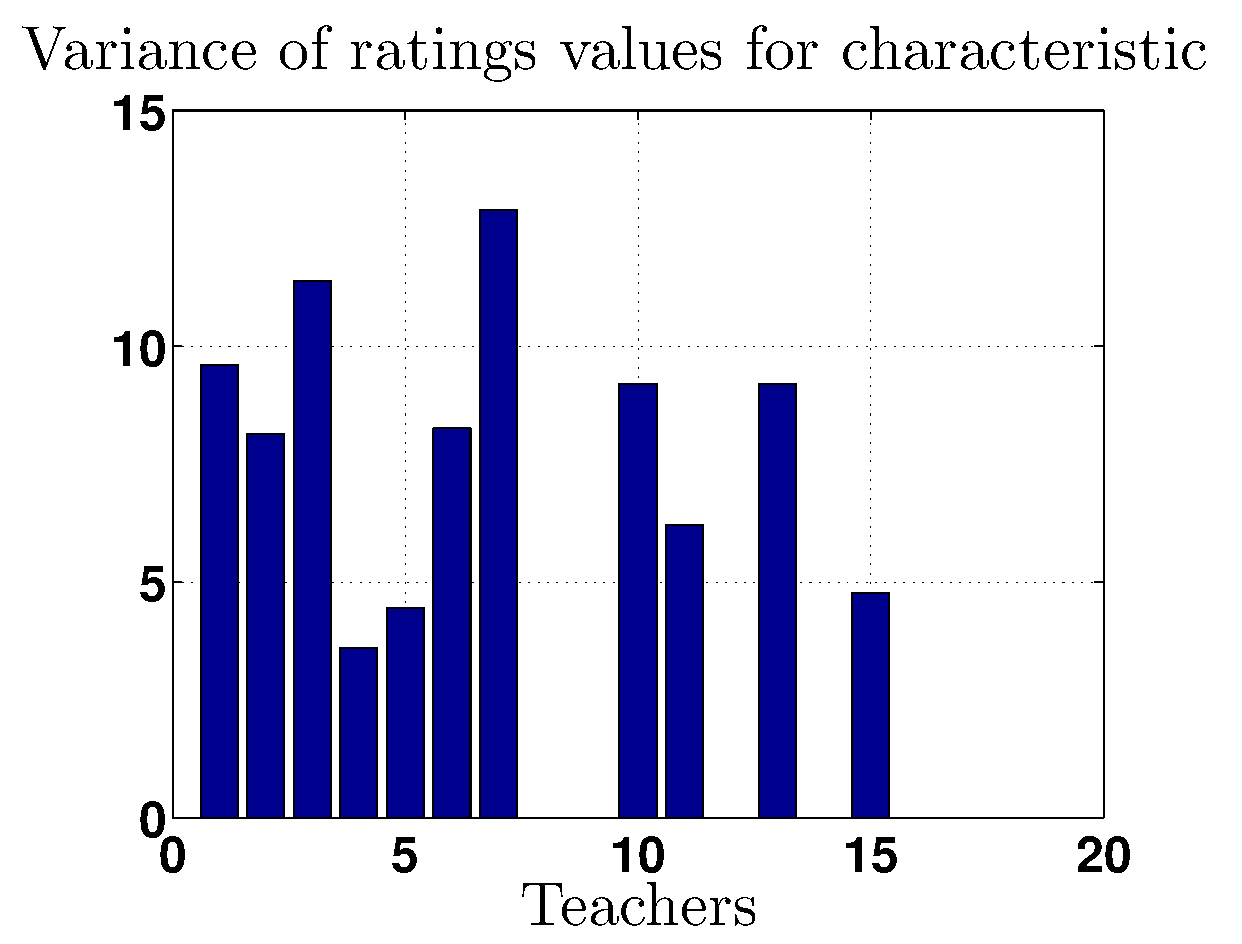
\includegraphics[width = 5cm]{noPreprocess/varTeachersC1.eps}
\end{subfigure}
\begin{subfigure}[b]{0.49\textwidth}
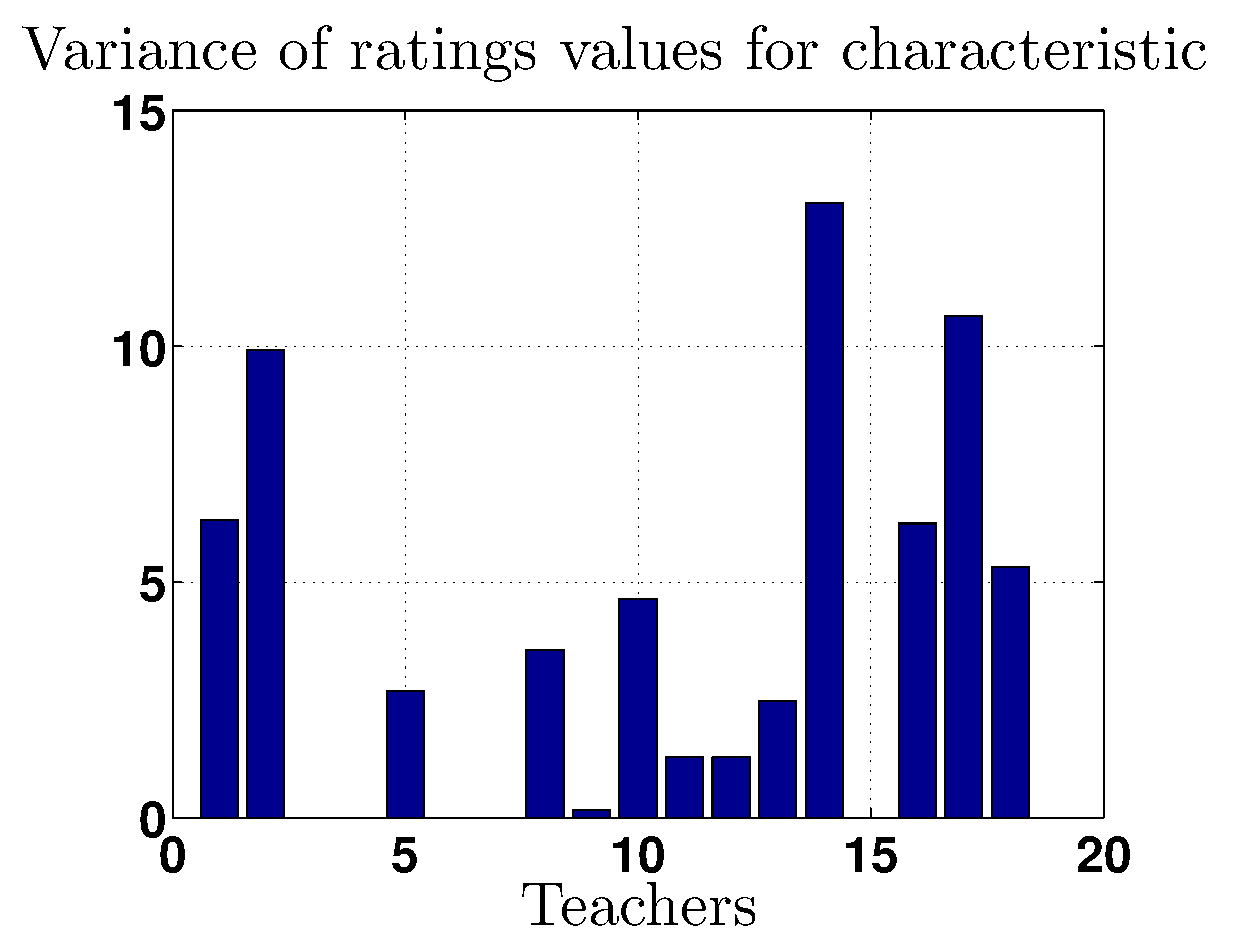
\includegraphics[width = 5cm]{noPreprocess/varTeachersC2.eps}
\end{subfigure}
\caption{Variance of ratings of teachers for mandatory and optional courses\label{var1}}
\end{figure}

Let's now compare with the weights obtained with different values of $k$. In figure \ref{noppk} we can see the influence of $k$ on weights. As expected, the weights lower as $k$ grows. We can see that the order of the weights does not change with $k$.

\begin{figure}[h!]
\centering
\begin{subfigure}[b]{0.48\textwidth}
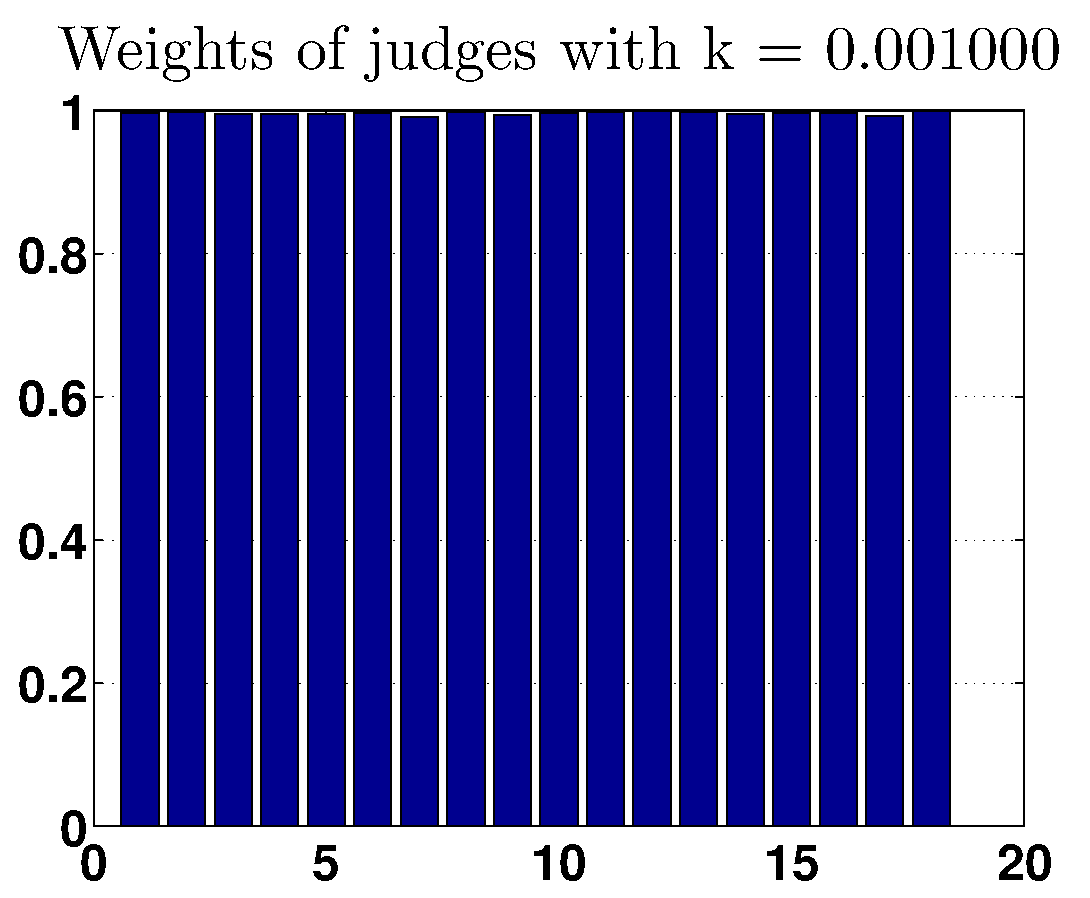
\includegraphics[width = 6cm]{noPreprocess/weightsk10.eps}
\end{subfigure}
\begin{subfigure}[b]{0.48\textwidth}
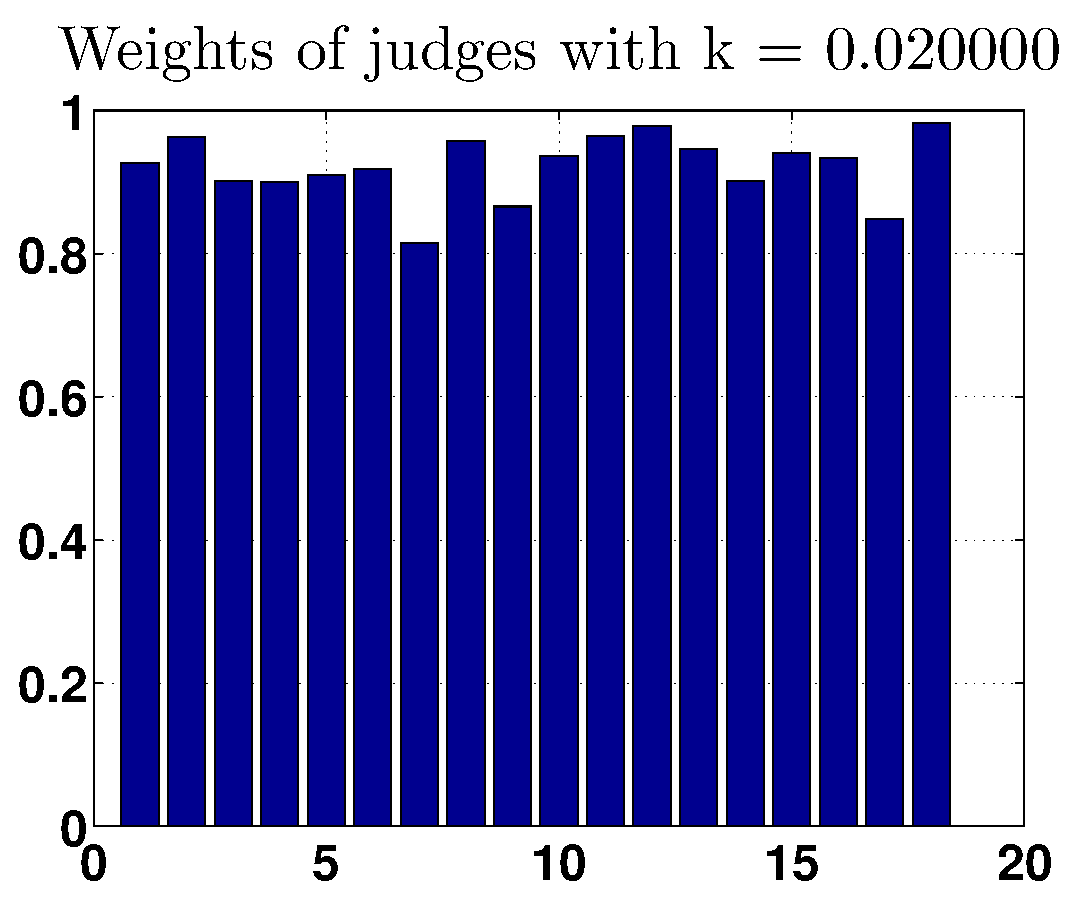
\includegraphics[width = 6cm]{noPreprocess/weightsk200.eps}
\end{subfigure}
\begin{subfigure}[b]{0.5\textwidth}
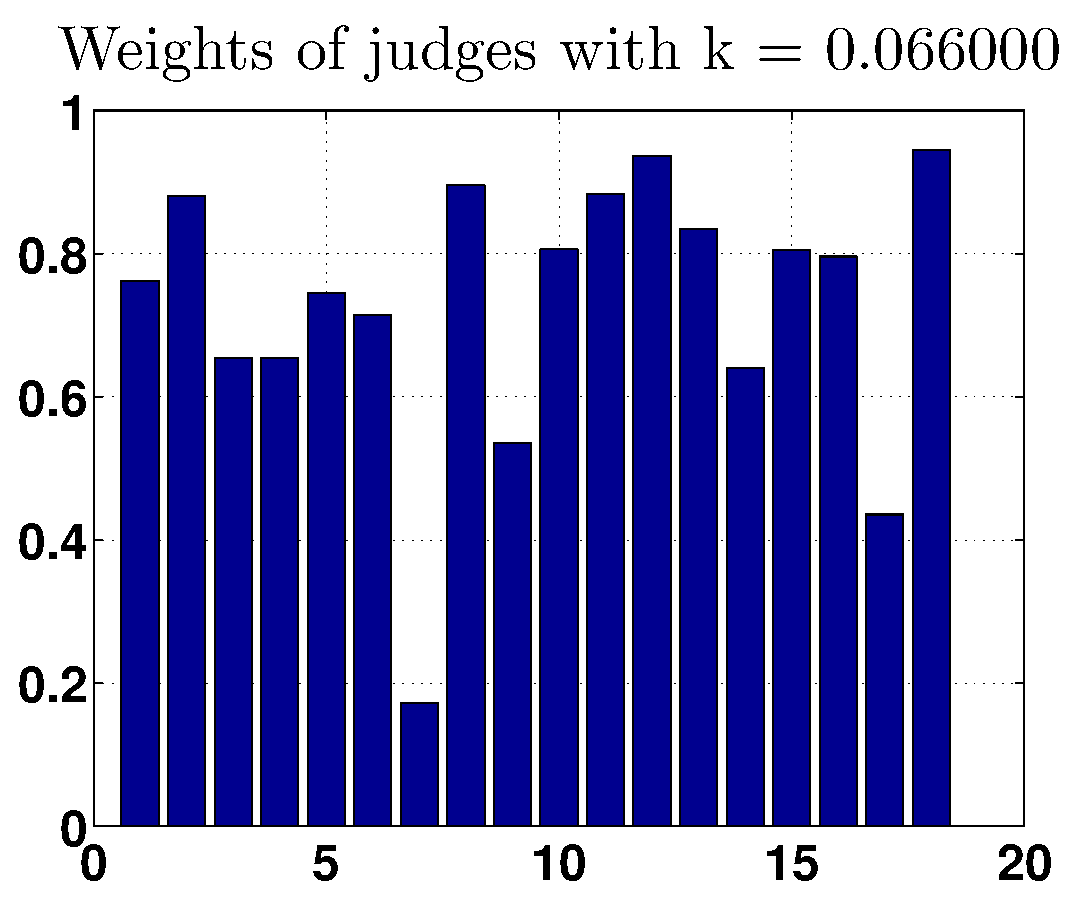
\includegraphics[width = 6cm]{noPreprocess/weightsk660.eps}
\end{subfigure}
\caption{\label{noppk}}
\end{figure}
We can see that there is a correlation between the mean rating and the weights. A mean value of ratings that is far from the values of mean rating for the other teacher will generally imply a lower weight, as it happens for teachers 3, 7 and 9. However, this is not a necessary condition since we can see that judge 17 has a pretty low weight although his mean is quite close from the others. We can also assess a link between high variance and low weight.\\

This argument justifies the normalizing of the ratings. Indeed, we will want to account only of the \textbf{order} of ratings. If a teacher is very demanding in some course and gives low marks to all his students, there is no reason to lower his weight as long as he remains consistent with the other teachers in the order he puts the students. Hence we will subtract the mean of each \textbf{course} to every rating. We also considered dividing the ratings by the standard deviation of the associated course since some teachers tend to vary more in the ratings they give. However we did not apply this idea because some potential cheaters with a very high variance could see their weight go up thanks to this processing.
\FloatBarrier

\subsection*{Preprocessing}
Here we have modified all the ratings of the courses so that their mean is 0. Let's note however that the final votes of the teachers do not necessarily have zero mean. \\
Let's now take the weights obtained with the maximum value of $k$ in figure (\ref{weightprocess}). Of course the weights are sensibly higher for the same values of $k$, which we need to increase in order to get some significant differentiation with the simple mean. We notice that the teachers with the lowest weights are not the same as before.

\begin{figure}[h!]
\centering
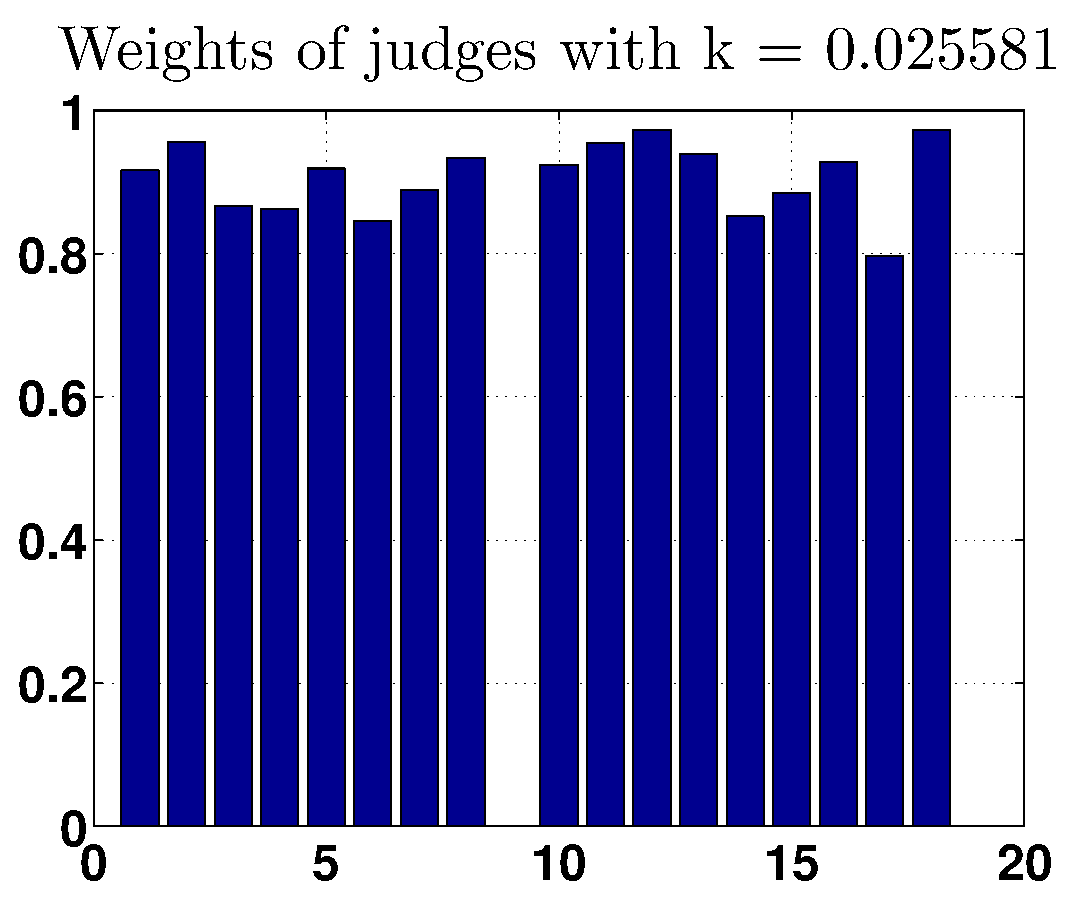
\includegraphics[width = 10cm]{preprocess/ppweightsk3f9a31ee697a4e60.eps}
\caption{\label{weightprocess}}
\end{figure}

When we look at the ratings given by the teachers with the highest and lowest weights (figure \ref{hlhist}), we notice that the lowest has given some very low marks. We assume that those are due to the student not passing the test seriously, since a rating of 1 out of 20 does not reflect the opinion of the teacher.\\
In order to say that the student really tried, he needs a grade of at least 8 out of 20. Hence we remove the ratings below that limit.

\begin{figure}[!h]
\centering
\begin{subfigure}[b]{0.48\textwidth}
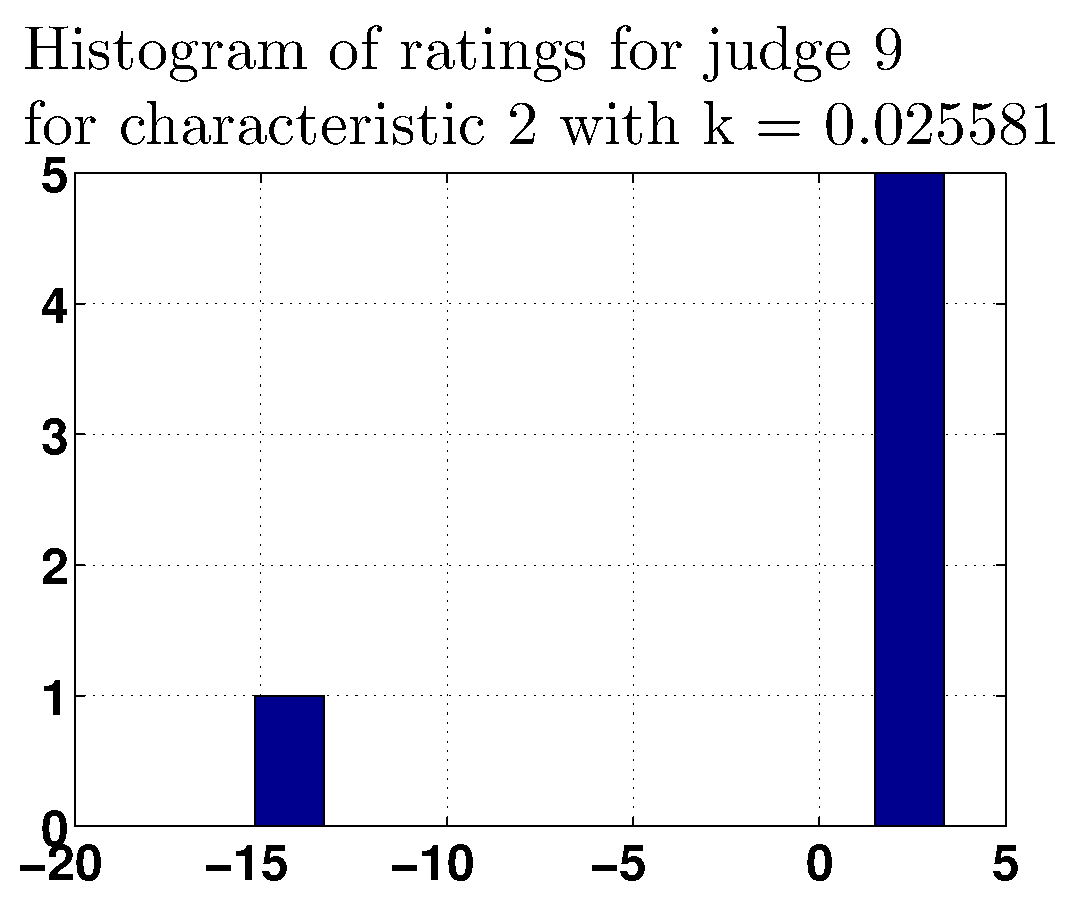
\includegraphics[width = 6cm]{preprocess/ppdistribLeastRelK406ff9f387c1ccacc2.eps}
\end{subfigure}
\begin{subfigure}[b]{0.48\textwidth}
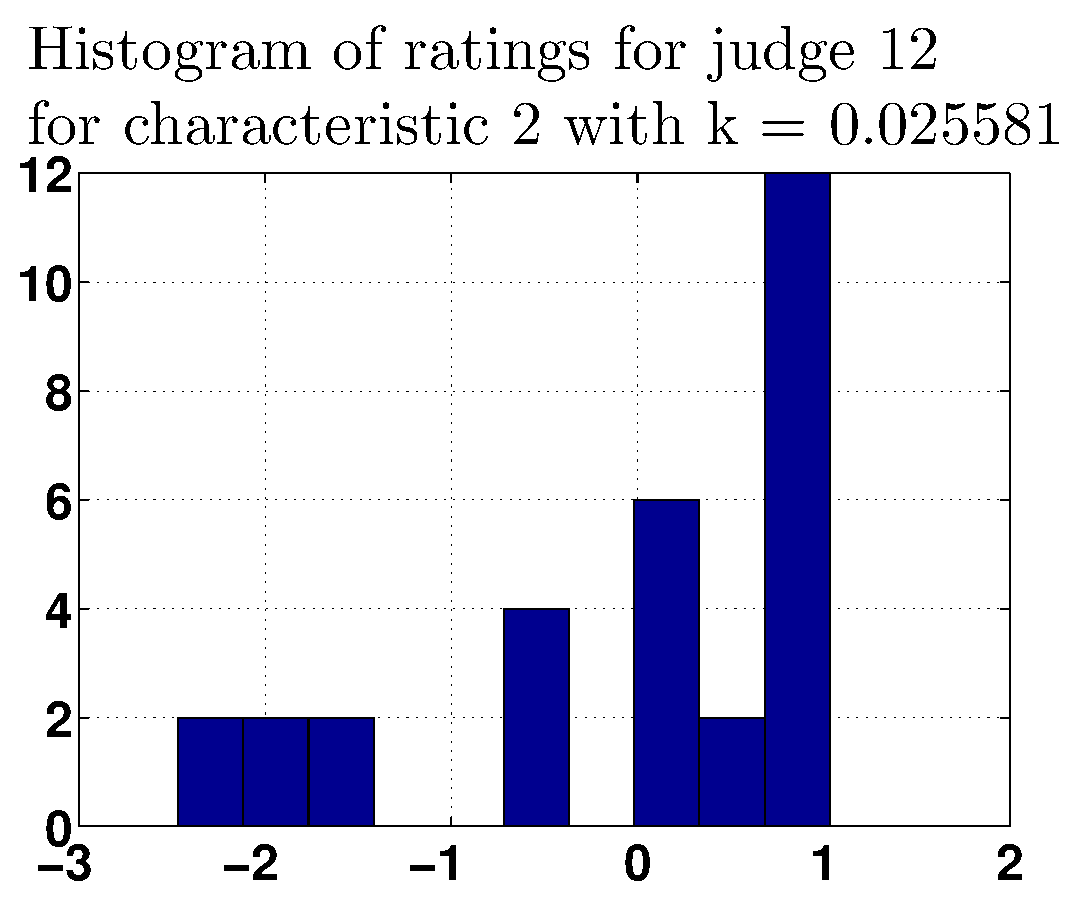
\includegraphics[width = 6cm]{preprocess/ppdistribMostRelK406ff9f387c1ccacc2.eps}
\end{subfigure}
\caption{\label{hlhist}Distribution of ratings for least reliable teacher(left) and most reliable teacher(right) for characteristic 2}
\end{figure}
\FloatBarrier

We can finally apply the iteration on the data. It can be seen in figure \ref{compRM} that the ratings do not evolve significantly. In general the difference between the reputation computed and the normal mean is not higher than half a point.\\
Although there are teachers whose weight is quite low (even one at zero), the fact that each student was rated by a lot of teachers reduces the possibility for great change.
\begin{figure}[!h]
\centering
\begin{subfigure}[b]{\textwidth}
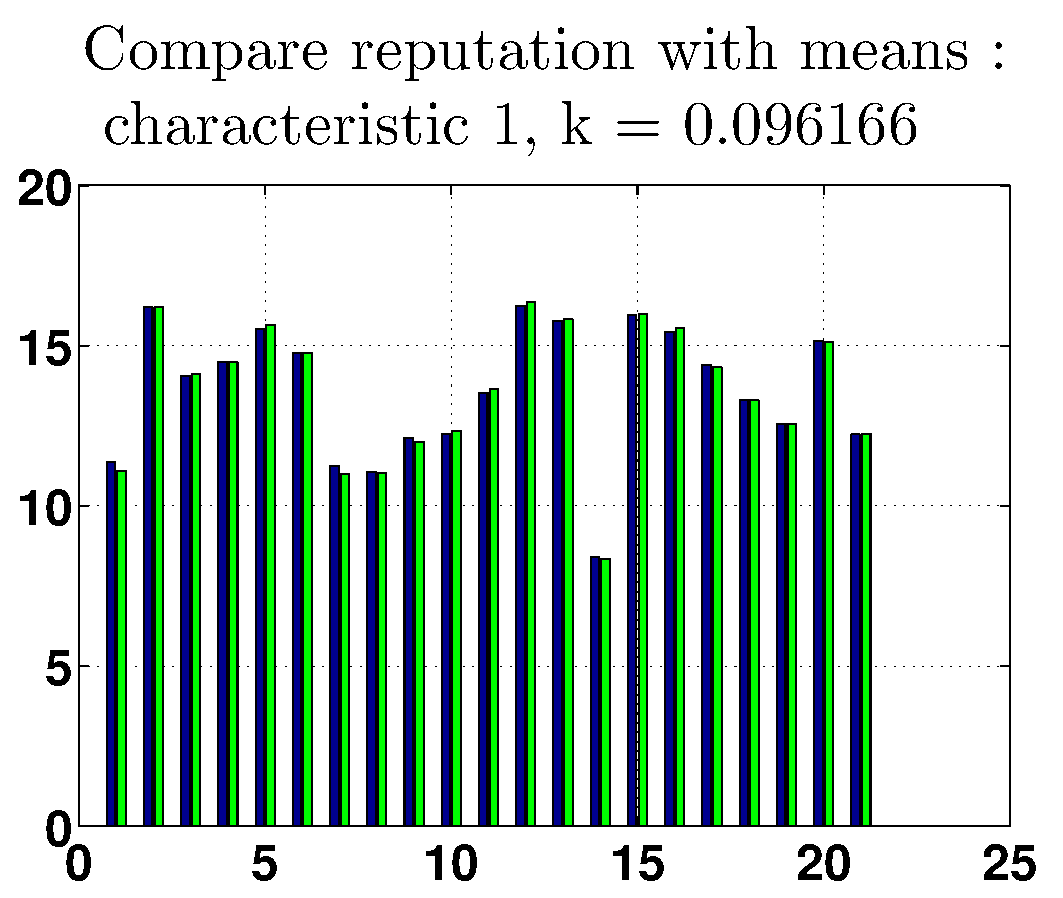
\includegraphics[width = 12cm]{preprocessSelect/ppscompareRepc1K3fb89e54e9211a25.eps}
\end{subfigure}
\begin{subfigure}[b]{\textwidth}
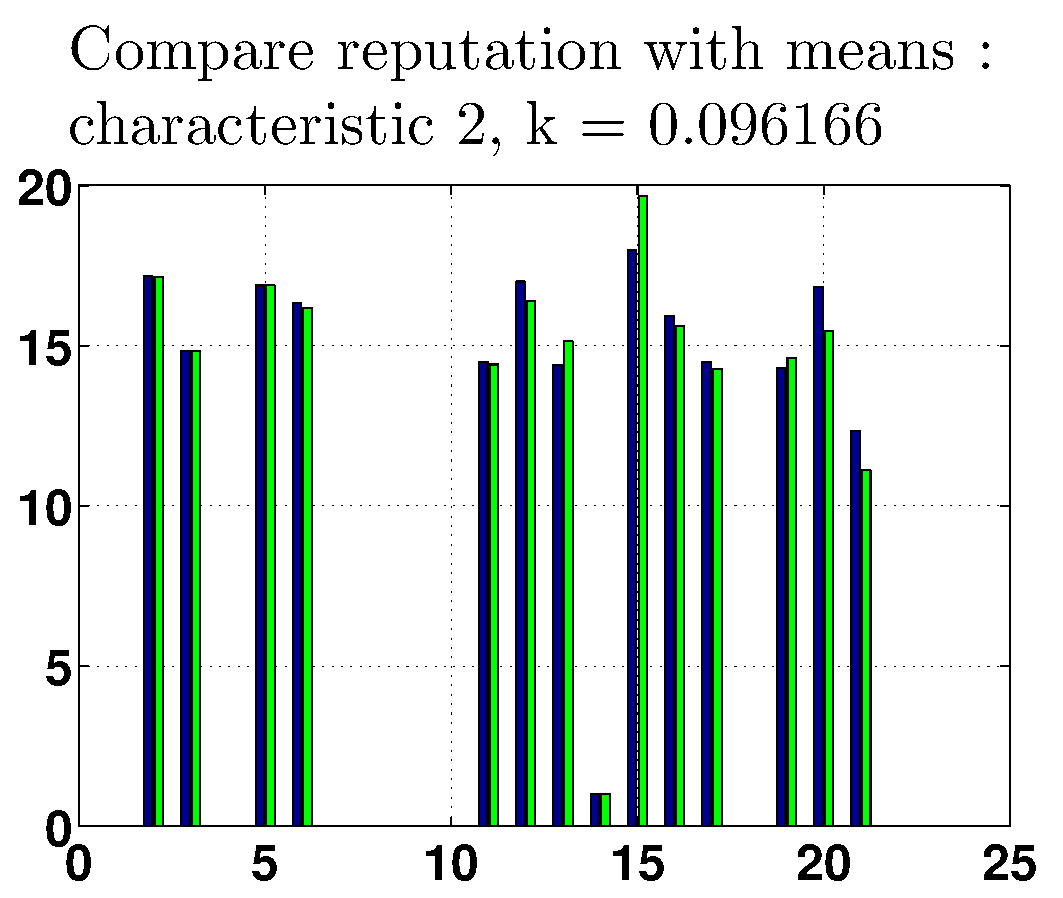
\includegraphics[width = 12cm]{preprocessSelect/ppscompareRepc2K3fb89e54e9211a25.eps}
\end{subfigure}
\caption{\label{compRM}Comparing the reputation and the mean ratings for all students}
\end{figure}
The difference between the ratings given and the reputations of the corresponding student for the least and most reliable teachers can be seen in figure \ref{diffLM}. As expected, the least reliable judge has a lot of differences quite high in absolute value. So does the most reliable judge, but he also has a lot of small differences, which help him keep a big weight.

\begin{figure}[!h]
\centering
\begin{subfigure}[b]{0.48\textwidth}
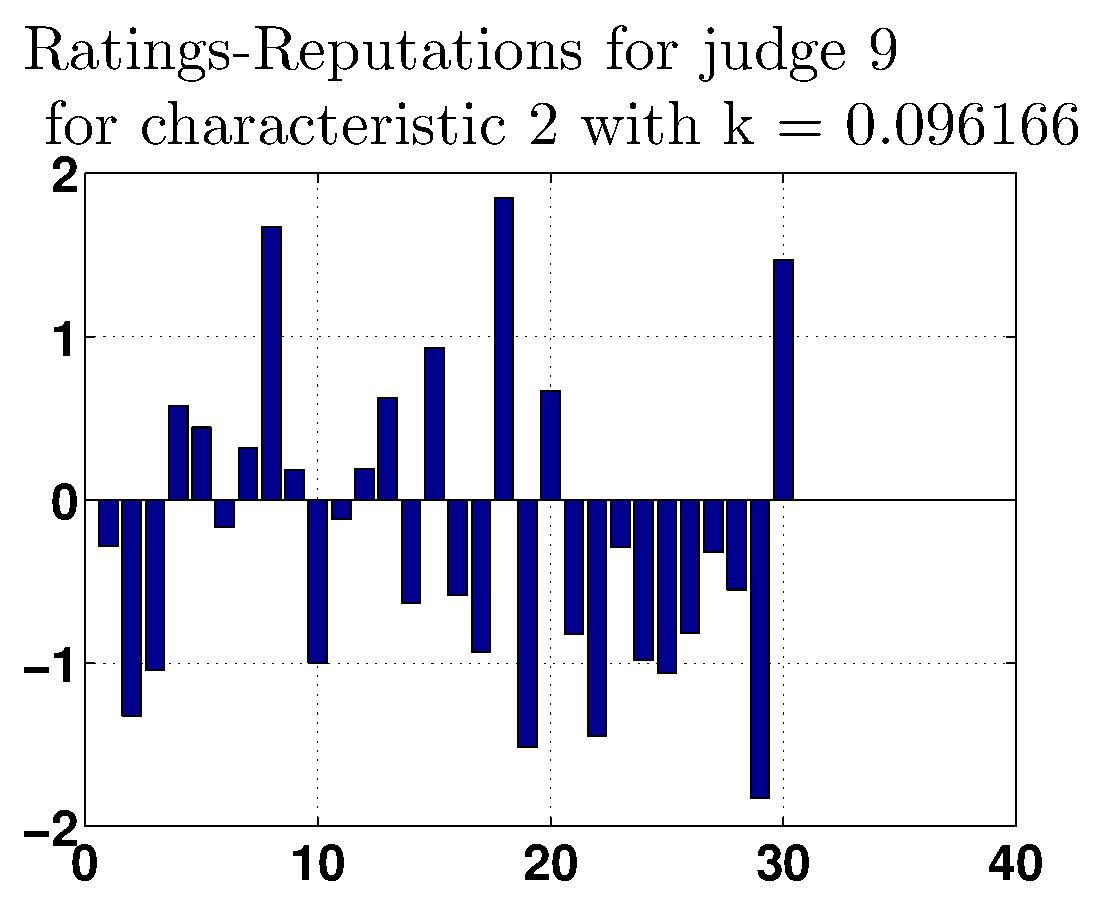
\includegraphics[width = 6cm]{preprocessSelect/ppsdiffRaReLeastK3fb89e54e9211a25c2.eps}
\end{subfigure}
\begin{subfigure}[b]{0.48\textwidth}
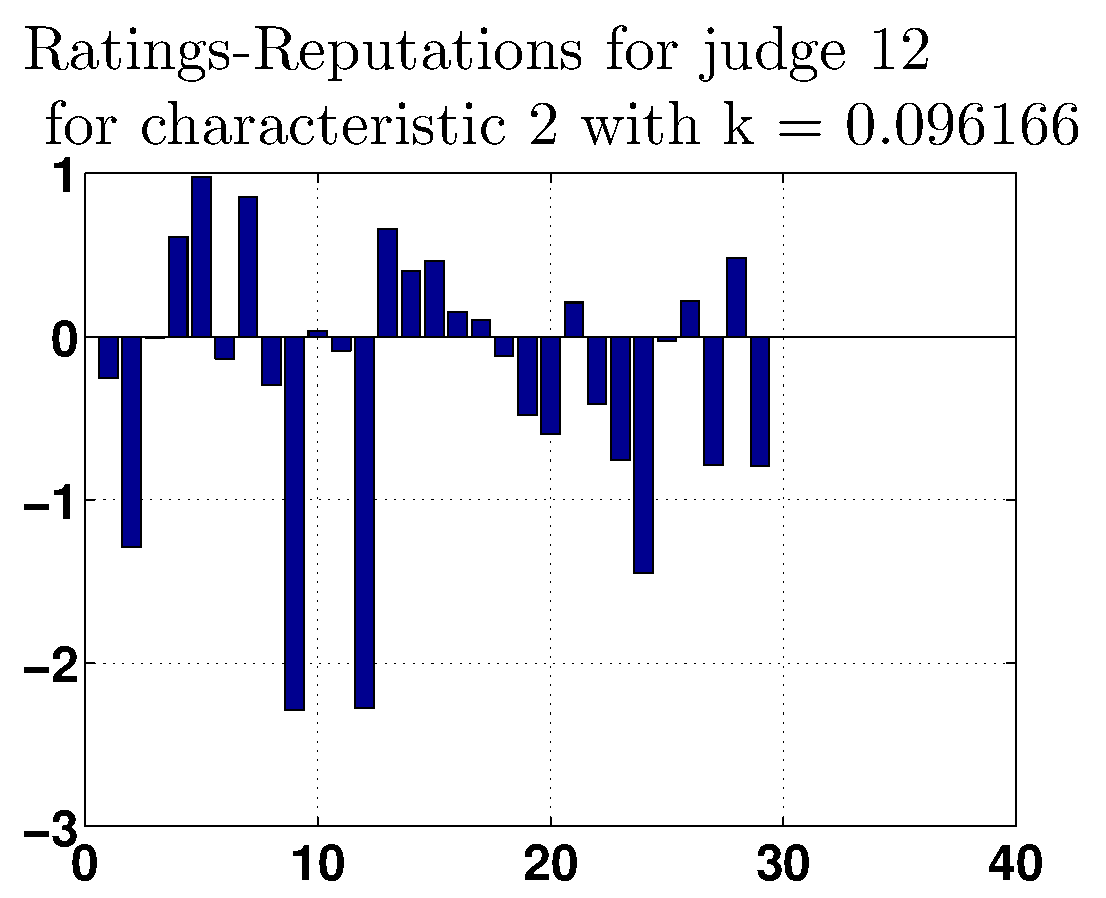
\includegraphics[width = 6cm]{preprocessSelect/ppsdiffRaReMostK3fb89e54e9211a25c2.eps}
\end{subfigure}
\caption{\label{diffLM}Difference between the ratings and the reputation for least(left) and most(right) reliable teachers}
\end{figure}

\subsection*{Influence of the number of ratings on weights}
In light of the latter results, we can ask ourselves what the influence of the number of ratings really is. Here we notice that low weights generally coincide with low number of ratings. This can be seen as the fact that the more a teacher gives interesting courses, the more he finds himself trusted by the system, and his mistakes on a few ratings are less important to his overall weight.
\begin{figure}
\centering
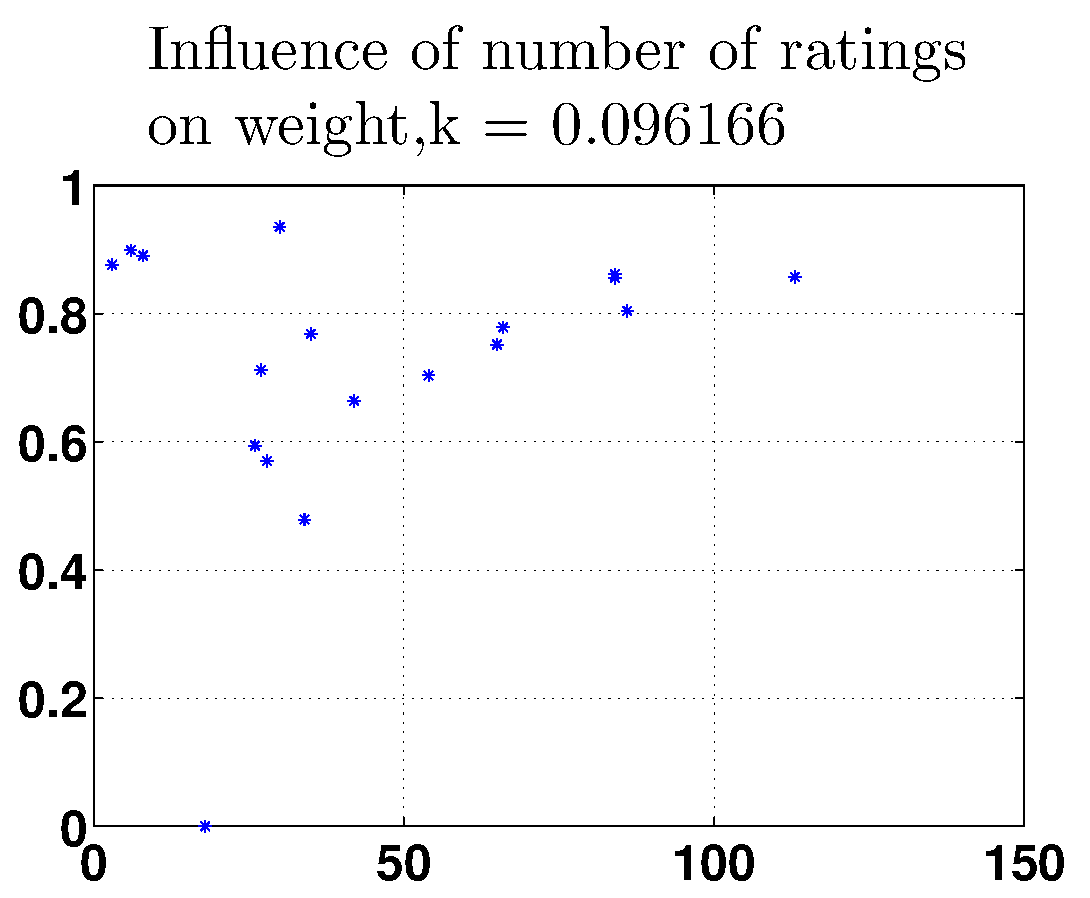
\includegraphics[width = 6cm]{preprocessSelect/ppsnumRatvsWK3fb89e54e9211a25.eps}
\caption{Influence of number of ratings on weight}
\end{figure}

\FloatBarrier

\subsection{Robustness tests}
In order to confirm the robustness of the iteration against cheaters, we performed three experiments on our data.\\
 First we added three stupid cheaters who would simply give a rating of $20$ to the favoured students and $8$, the minimum acceptable note for disfavoured students. The cheaters were correctly detected and their weight immediately set to zero, hence not modifying the final reputations.\\
 Then we added three more subtle cheaters who, rather than giving $20$ and $8$ gave $19$ and $9$. They were also detected, but here the value of $k$ was larger.\\
 Finally we mixed the two behaviours, using one stupid cheater and two subtle cheaters. This time the weight of the stupid cheater was set to zero, but it was not the case for the subtle cheaters, because the $k$ couldn't be as high as in the latter case without causing some weights to be negative. In that case, we find the difference between the former reputation and the new reputation to be significant.\\
 
In figure \ref{weightch} we can see from left to right the weights for the three scenarios described above. We can see that in the third case the weights of the smart cheaters are non-zero but are still lower than the average.

\begin{figure}
\begin{subfigure}[b]{0.32\textwidth}
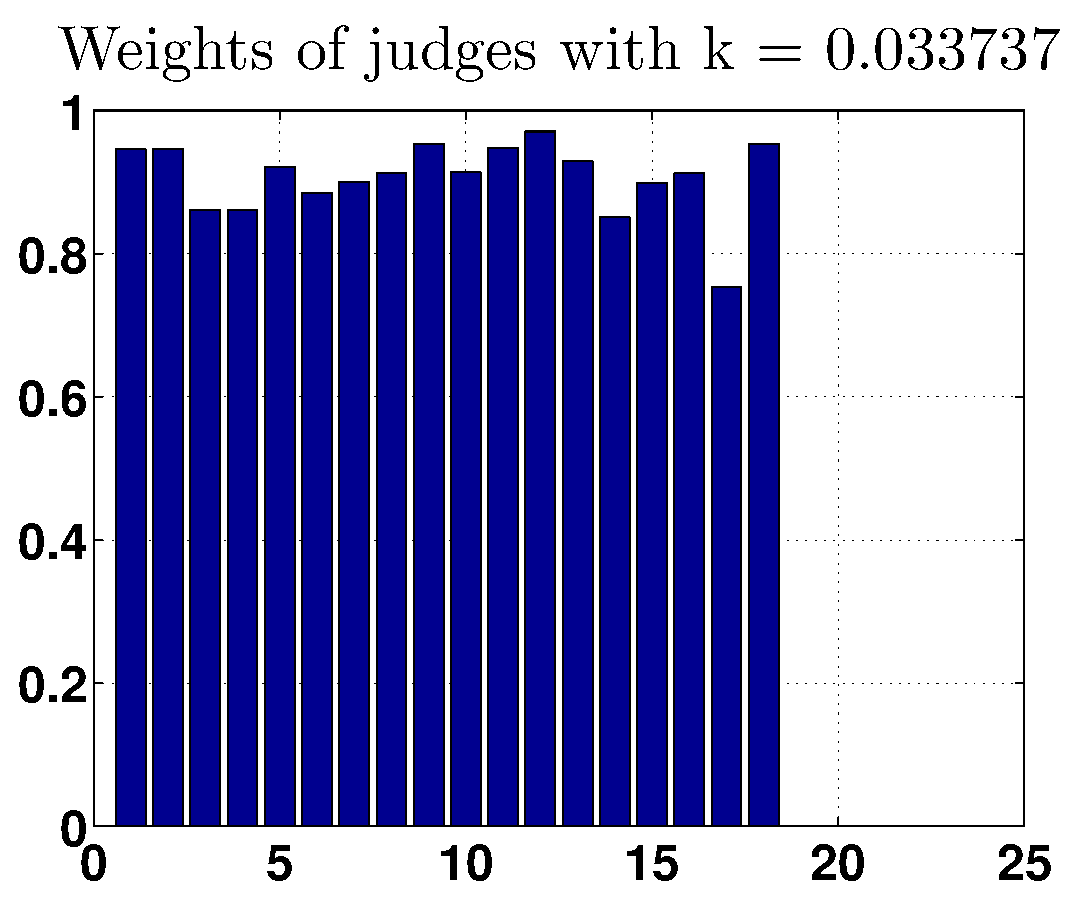
\includegraphics[width = 4cm]{cheaters/chweightsStupid.eps}
\end{subfigure}
\begin{subfigure}[b]{0.32\textwidth}
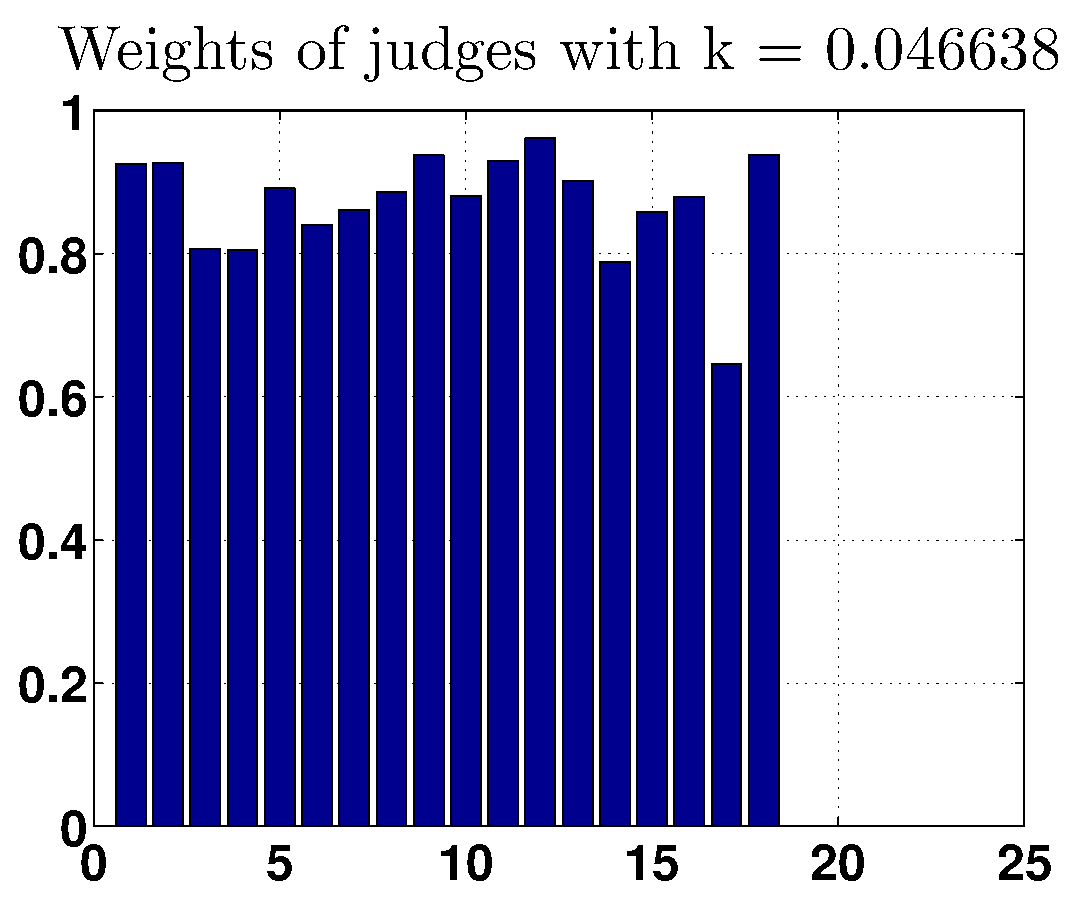
\includegraphics[width = 4cm]{cheaters/chweightsSmart.eps}
\end{subfigure}
\begin{subfigure}[b]{0.32\textwidth}
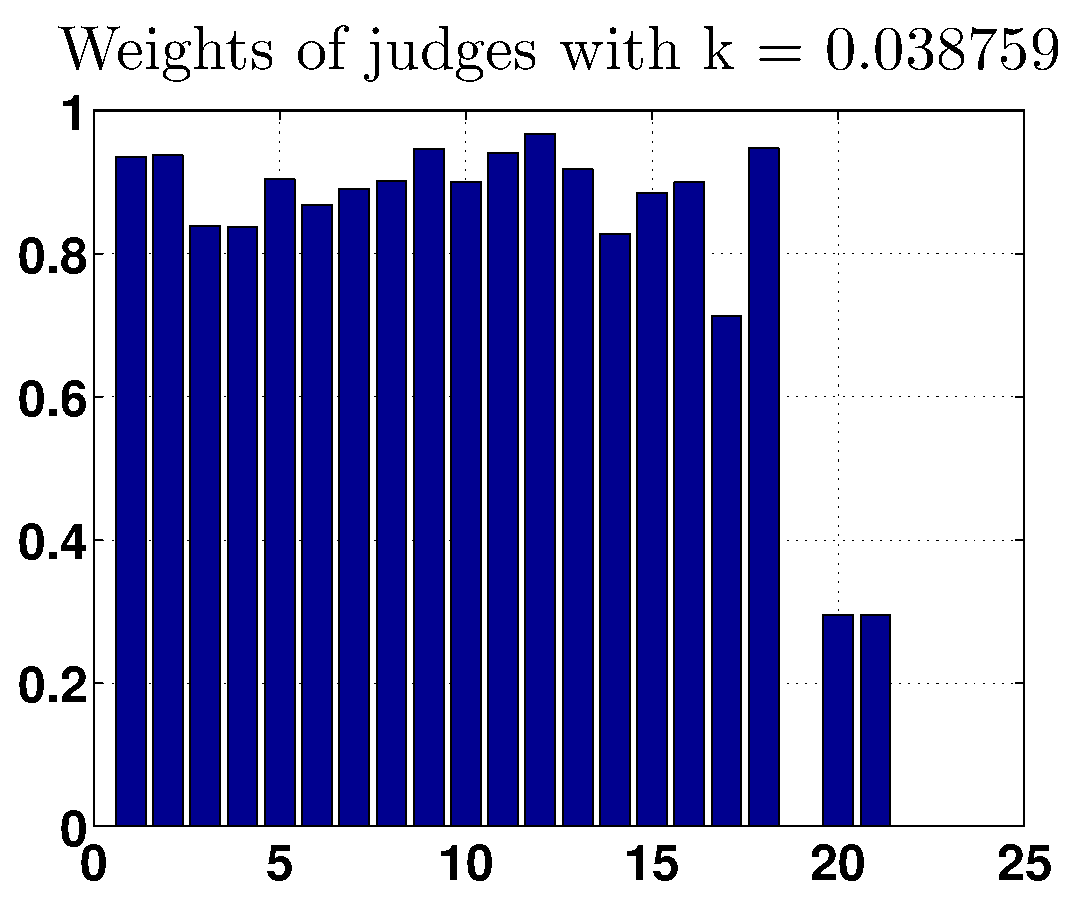
\includegraphics[width = 4cm]{cheaters/chweightsMix.eps}
\end{subfigure}
\caption{Weights for the three scenario of cheaters\label{weightch}}
\end{figure}

In figure \ref{finalCheat} we can see a comparison of initial reputation, reputation after cheaters and reputation computed using the usual mean for the three scenarios. The first five students are the favoured students and the fifteen next are disfavoured. While the two first scenarios do not exhibit a great difference between the initial and final reputations, the third case does change significantly. We can see that in all three cases the final reputation (in green) is closer to the initial reputation (in blue) than the mean of the ratings (in red).
\begin{figure}
\centering
\begin{subfigure}[b]{0.49\textwidth}
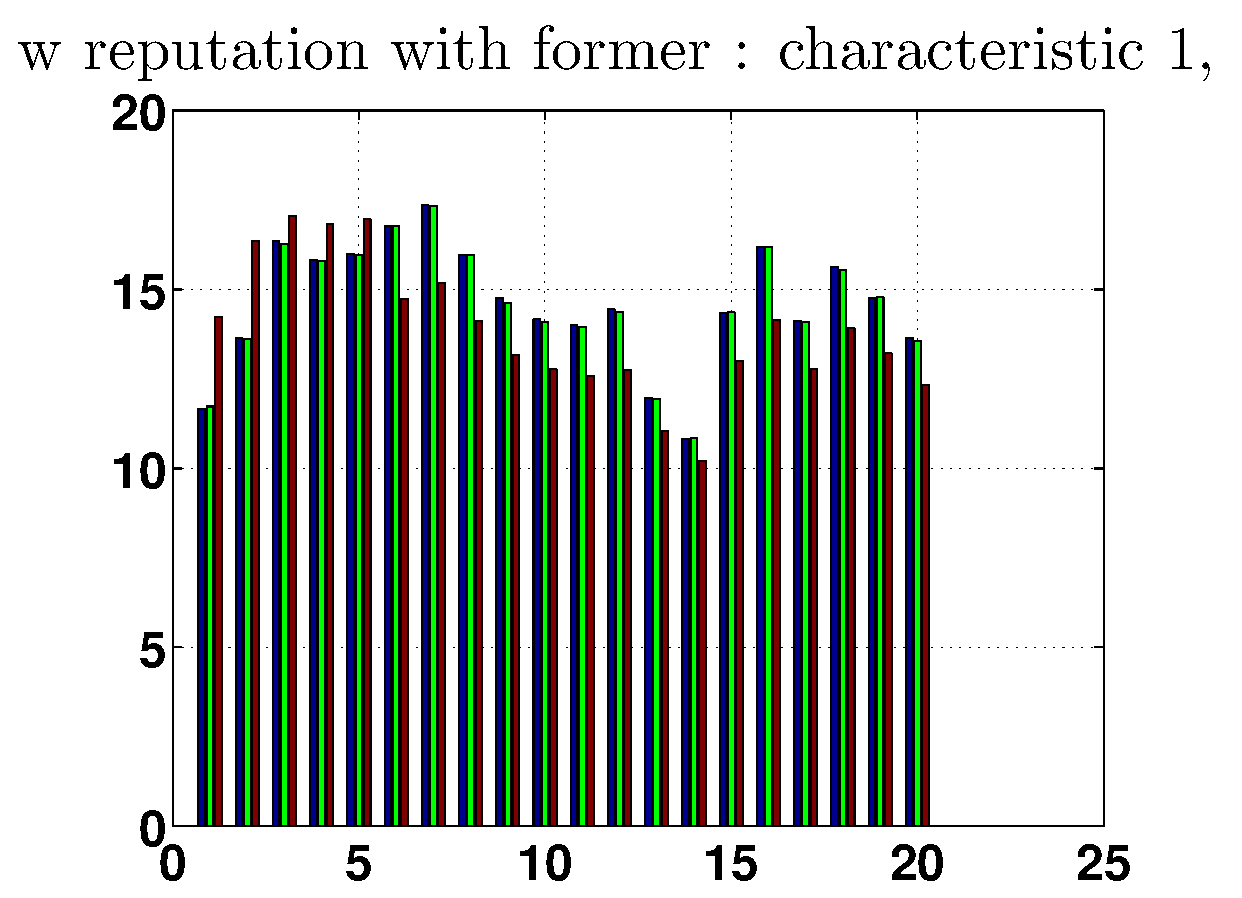
\includegraphics[width = 7.5cm]{cheaters/chcompareRepStupidc1.eps}
\end{subfigure}
\begin{subfigure}[b]{0.49\textwidth}
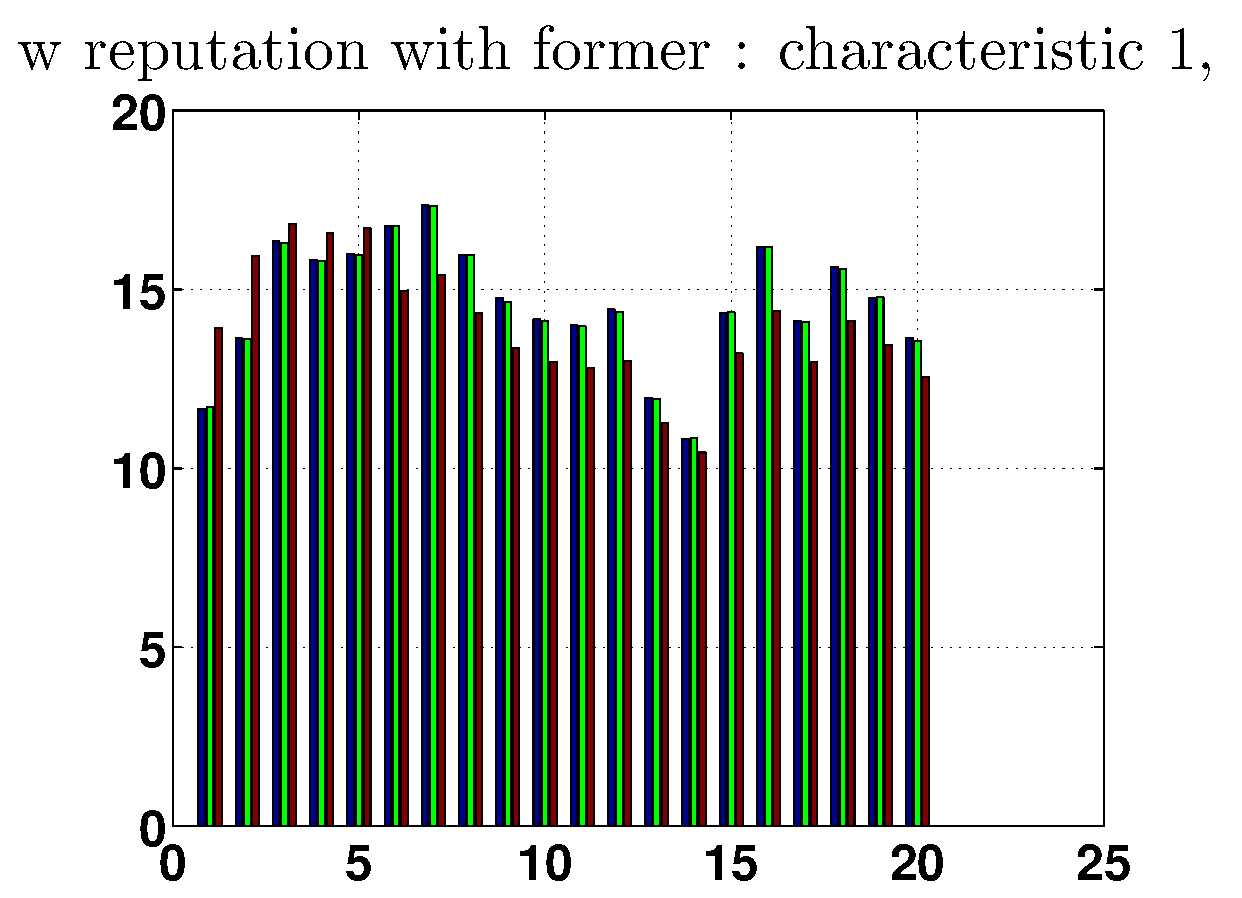
\includegraphics[width = 7.5cm]{cheaters/chcompareRepSmartc1.eps}
\end{subfigure}
\begin{subfigure}[b]{0.49\textwidth}
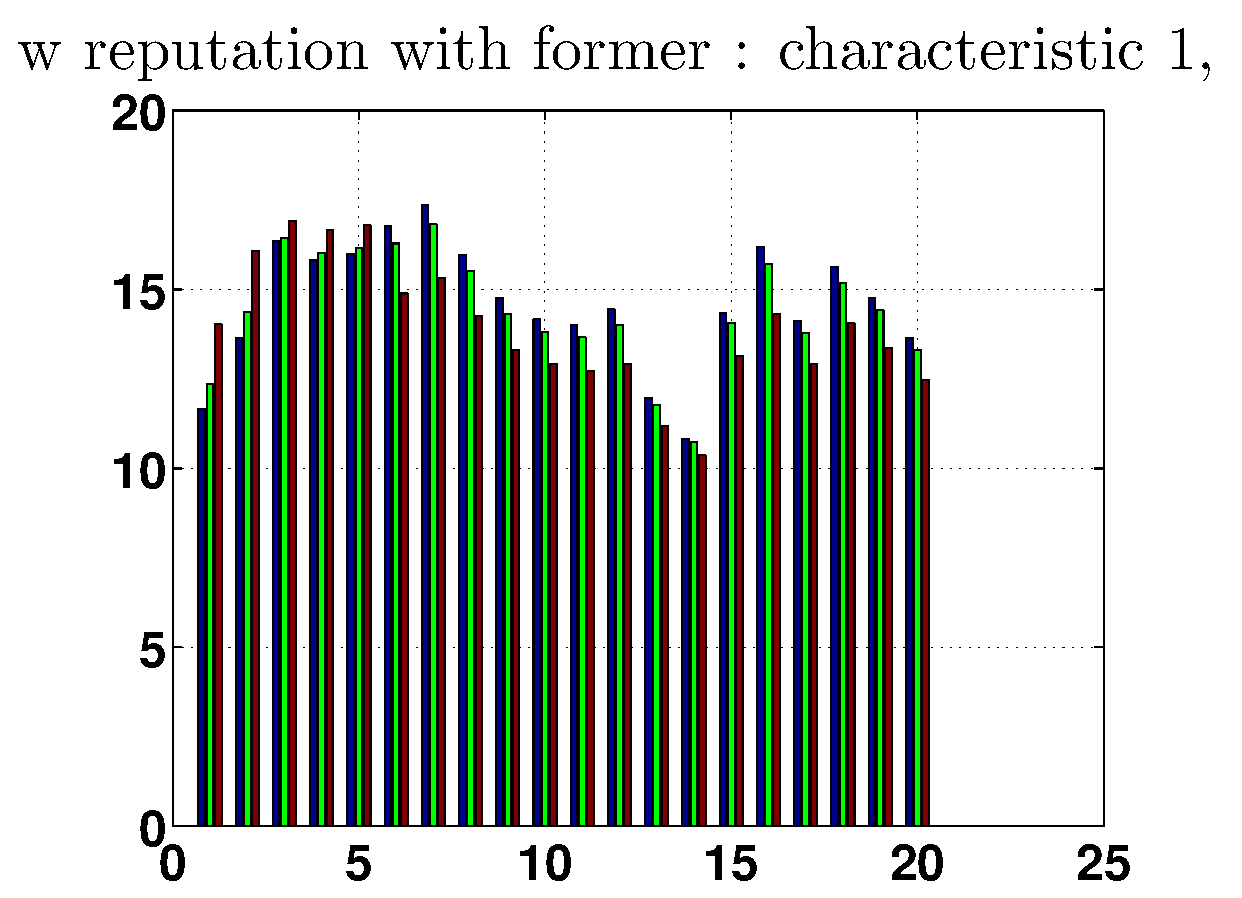
\includegraphics[width = 7.5cm]{cheaters/chcompareRepMixc1.eps}
\end{subfigure}
\caption{\label{finalCheat}Comparison of initial reputation, reputation after cheaters and reputation computed using the usual mean for the three scenarios}
\end{figure}


\section{Application to Hotels}

We were given the scores of the hotels in the subset database of TripAdvisor \footnote{http://times.cs.uiuc.edu/~wang296/Data/}. Here we did  expect to have significant results on the reliability of some users. Then we observe the robustness of the algorithm by injecting spammers.

\subsection{Preprocessing}
Our experiment concerns a data set of 12773 hotels evaluated by 1169410 users on 10 characteristics and ranging from 1 to 5. But we select a subset of this data set. Indeed, the hotels that have been evaluated by 1 user are not of interest us, as users who would have voted for a hotel. This allows us to reduce the data set to a smaller and more usable set. To further reduce the data we have selected the users who voted for at least 4 hotels. The subset includes 305 hotels evaluated by 20024 users on 9 characteristics. We also noticed that the dataset is extremely sparse.

\subsection{Analyse results} 

After the iteration we observe a distribution of weights illustrated at figure (\ref{fig:hotel:initial_weights}). We note that most users are consistent and thus the weights are high. Unfortunately, we do not detect a specific behaviour.

\begin{figure}[!h]
\centering
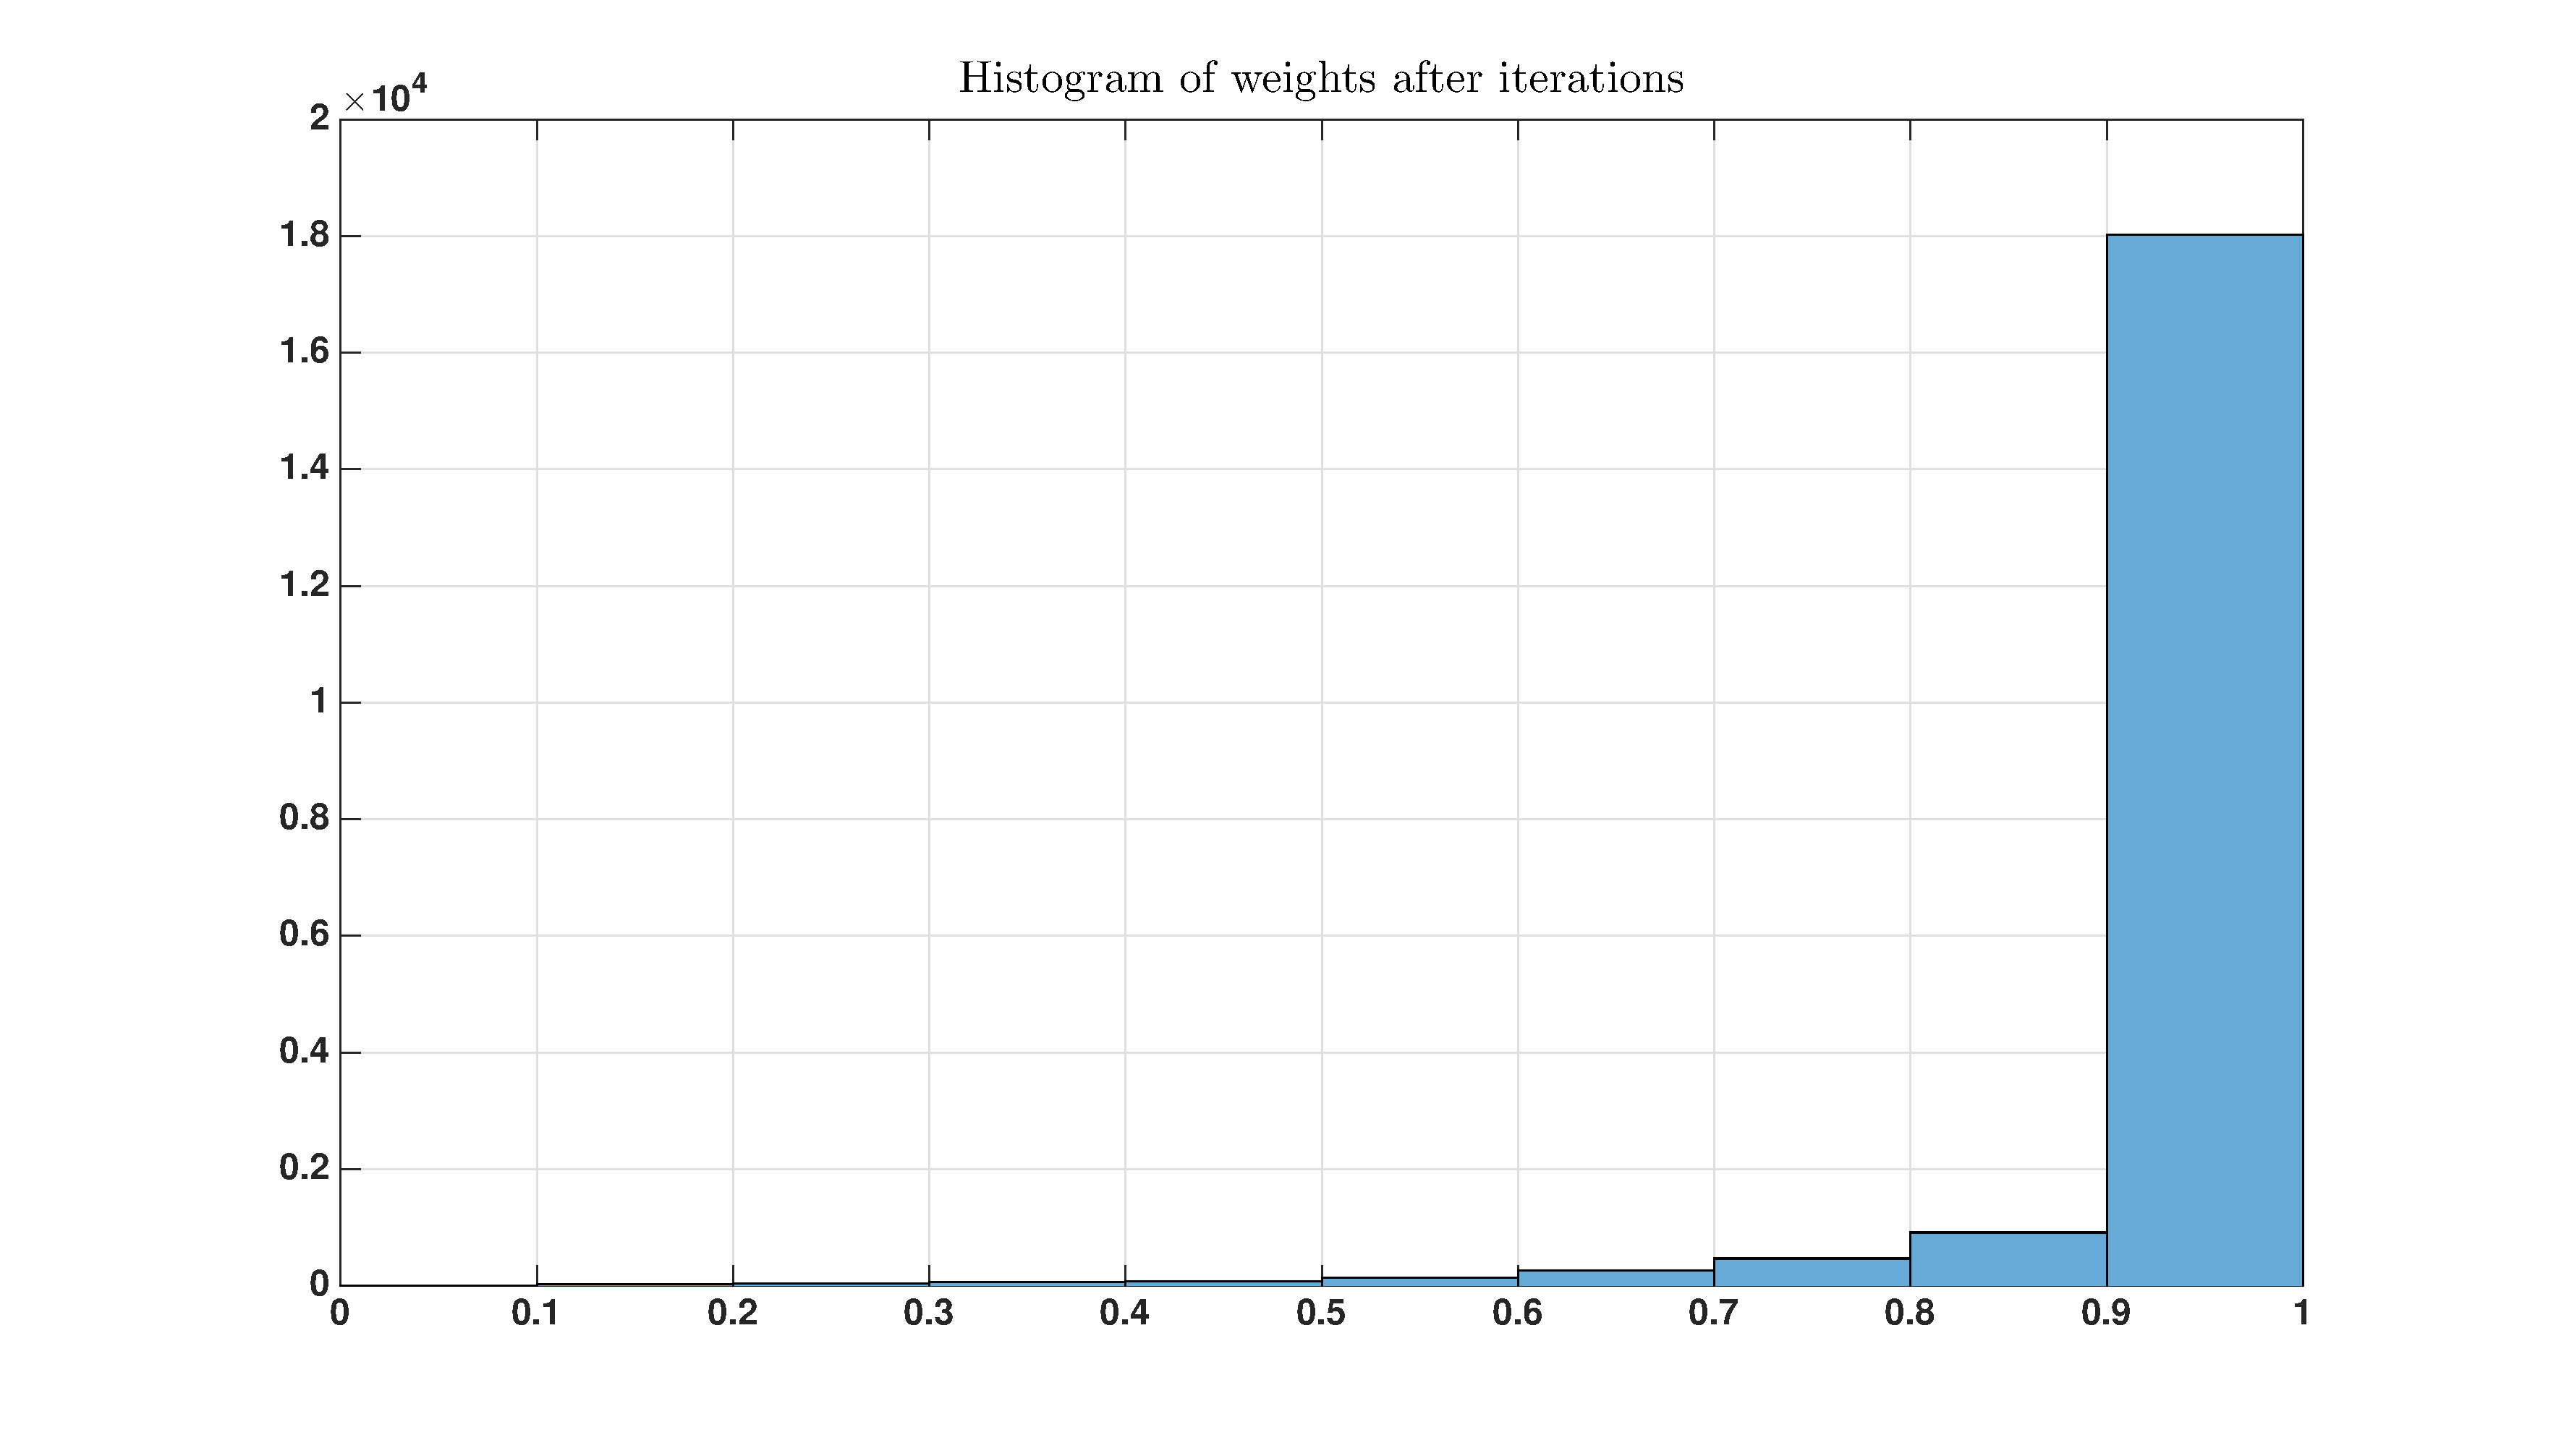
\includegraphics[width = 0.8\textwidth]{hotels/initial_weights.eps}
\caption{\label{fig:hotel:initial_weights} Distribution of weights after iterations}
\end{figure}

\subsection{Robustness tests}

In order to simulate the robustness of our algorithm, two types of behaviour are analysed in the sequel: first, judges that give random evaluations, and second, spammers that try to improve the reputation of their preferred hotel.

\subsubsection*{Robustness against random raters}
We added to the original data set 2000 judges evaluating randomly some hotels. In that manner, 10\% of the judges give random evaluations. The figure (\ref{fig:hotel:random_cheaters}) illustrate the distribution of weights after iteration with and without spammers.

\begin{figure}[!h]
\centering
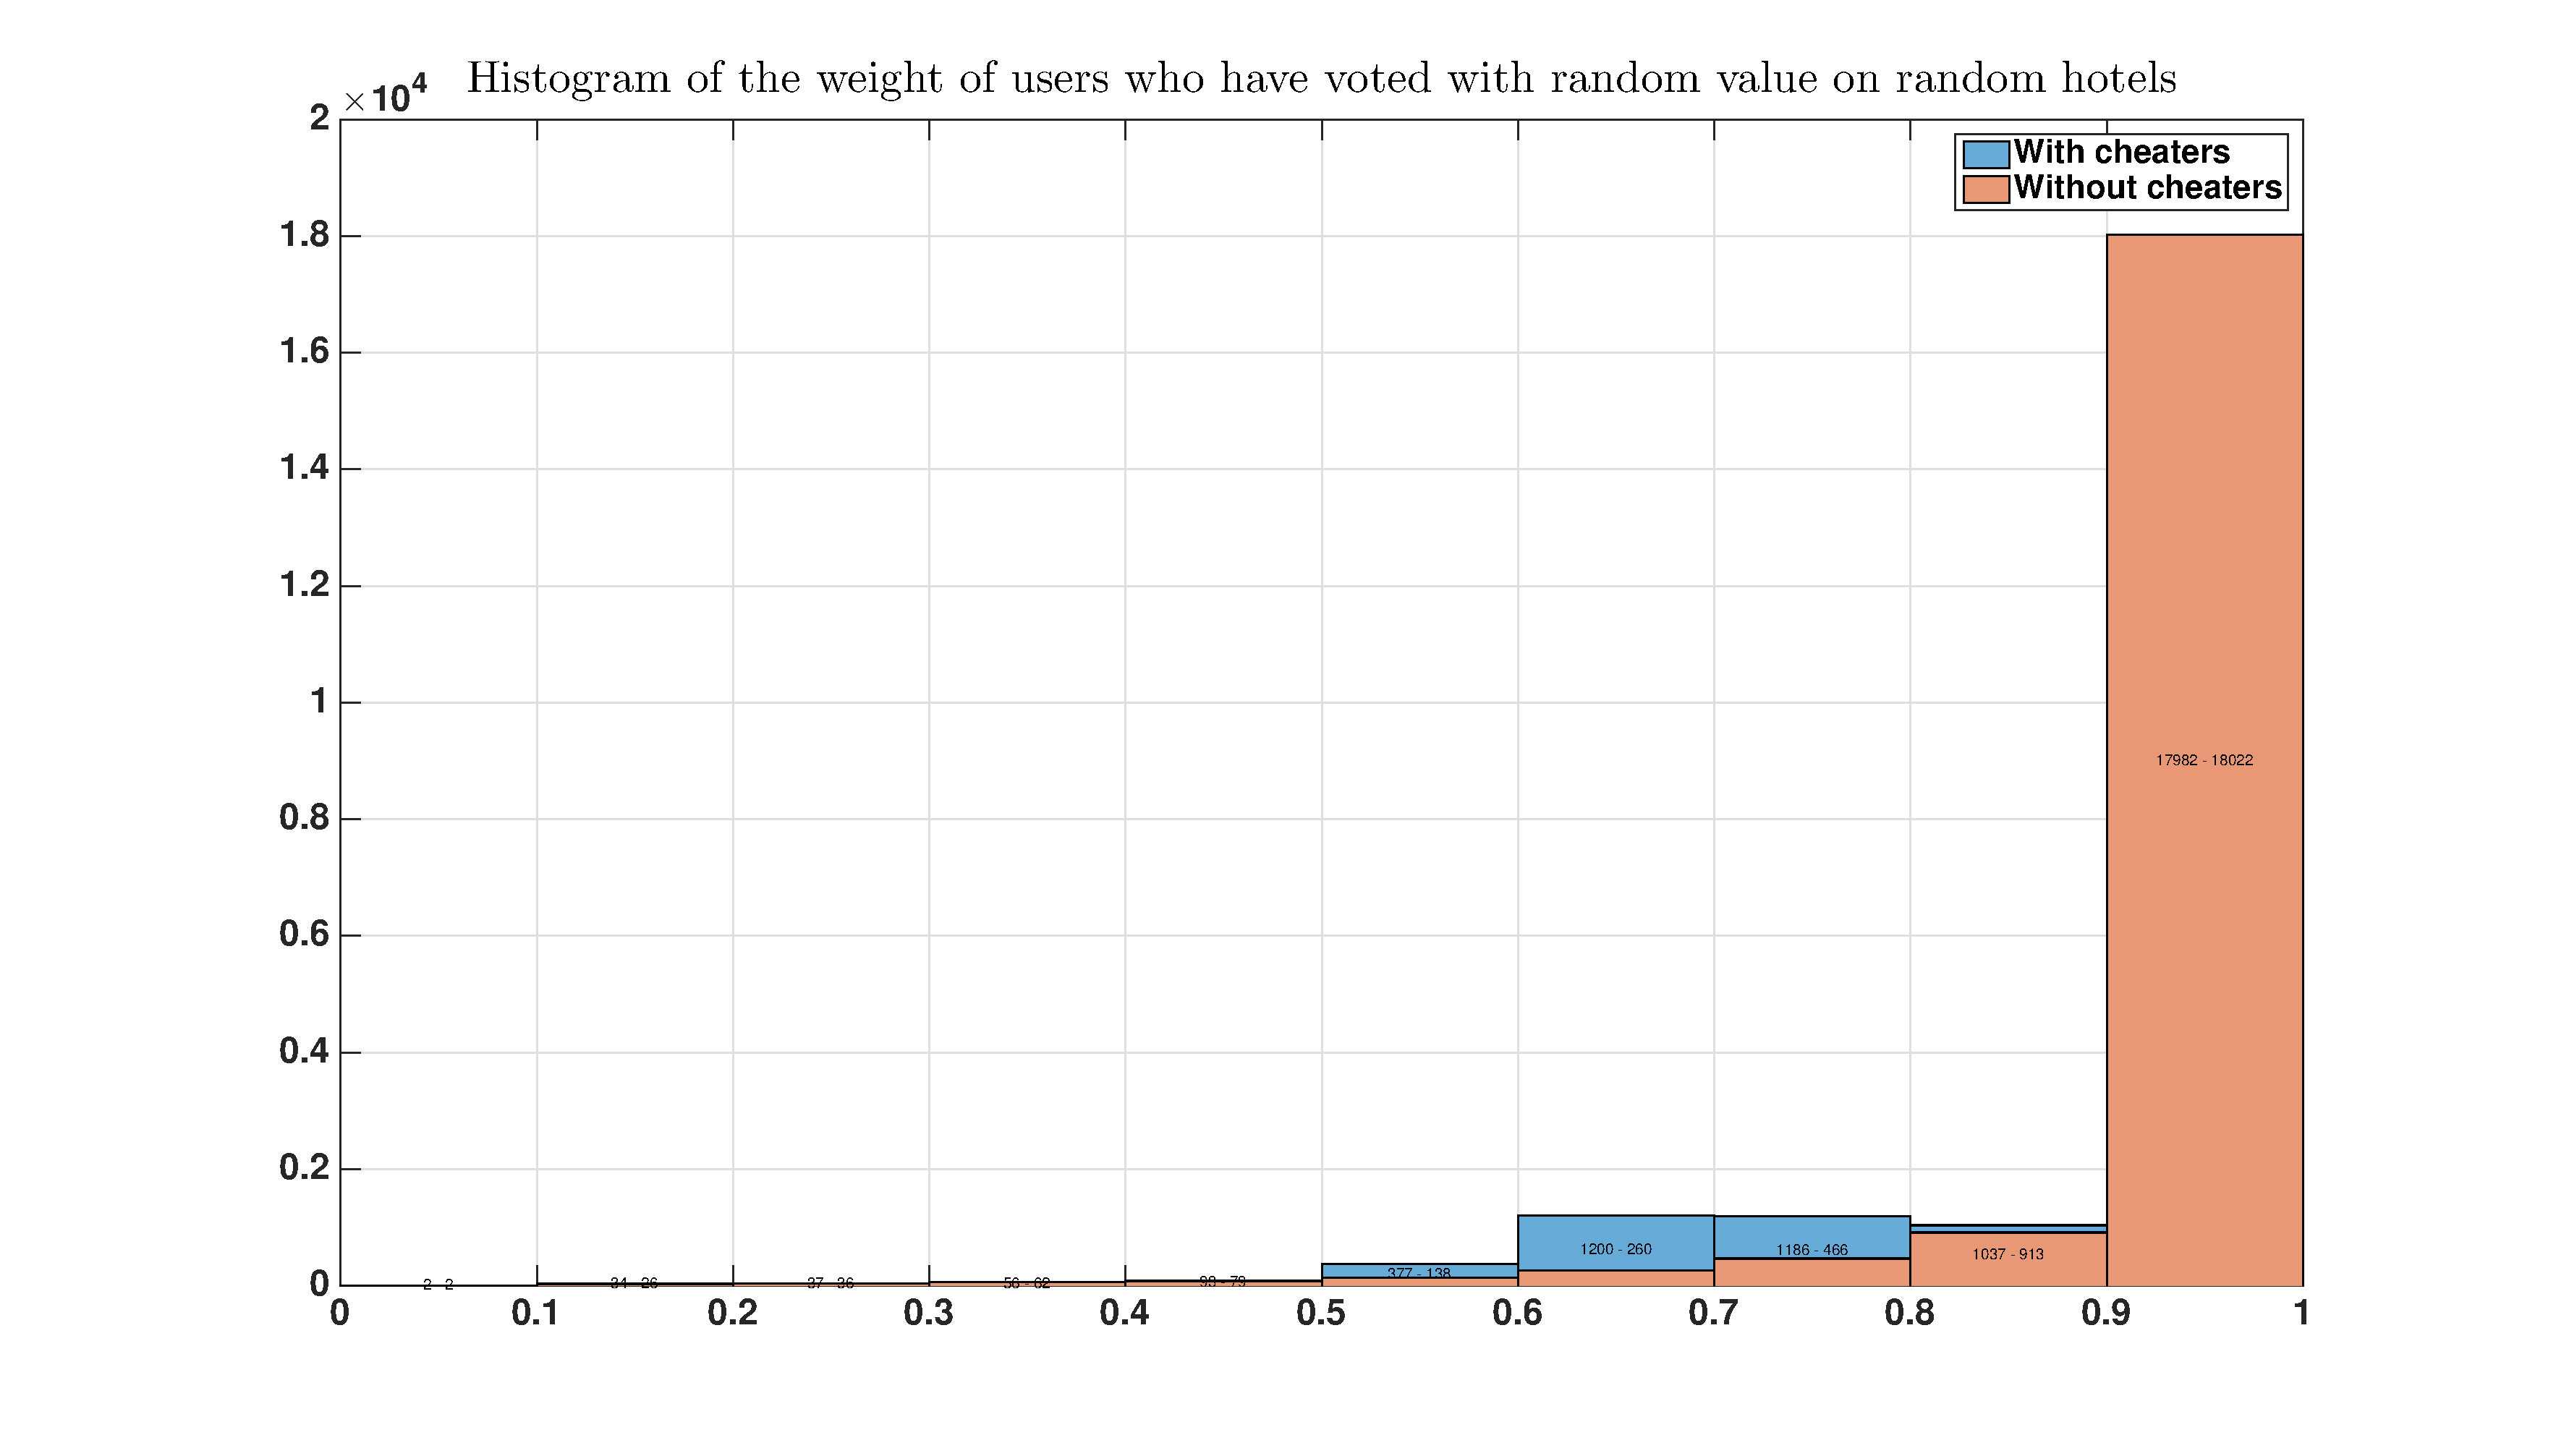
\includegraphics[width = \textwidth]{hotels/random_cheaters.eps}
\caption{\label{fig:hotel:random_cheaters} Distribution of weights after iterations with and without spammers}
\end{figure}

Weights spammers are in this case still high. This is probably because the data are very sparses and it is difficult to compare the spammers to other users if the notes are distributed consistent manner. Spammers are identifiable at the expense of some other users.

\subsubsection*{Robustness against spammers}

We now added to the original data set 20 spammers giving always 0 except for their preferred hotel, which they rated 5. The figure (\ref{fig:hotel:not_random_cheaters}) illustrate the distribution of weights after iteration with and without spammers.

\begin{figure}[!h]
\centering
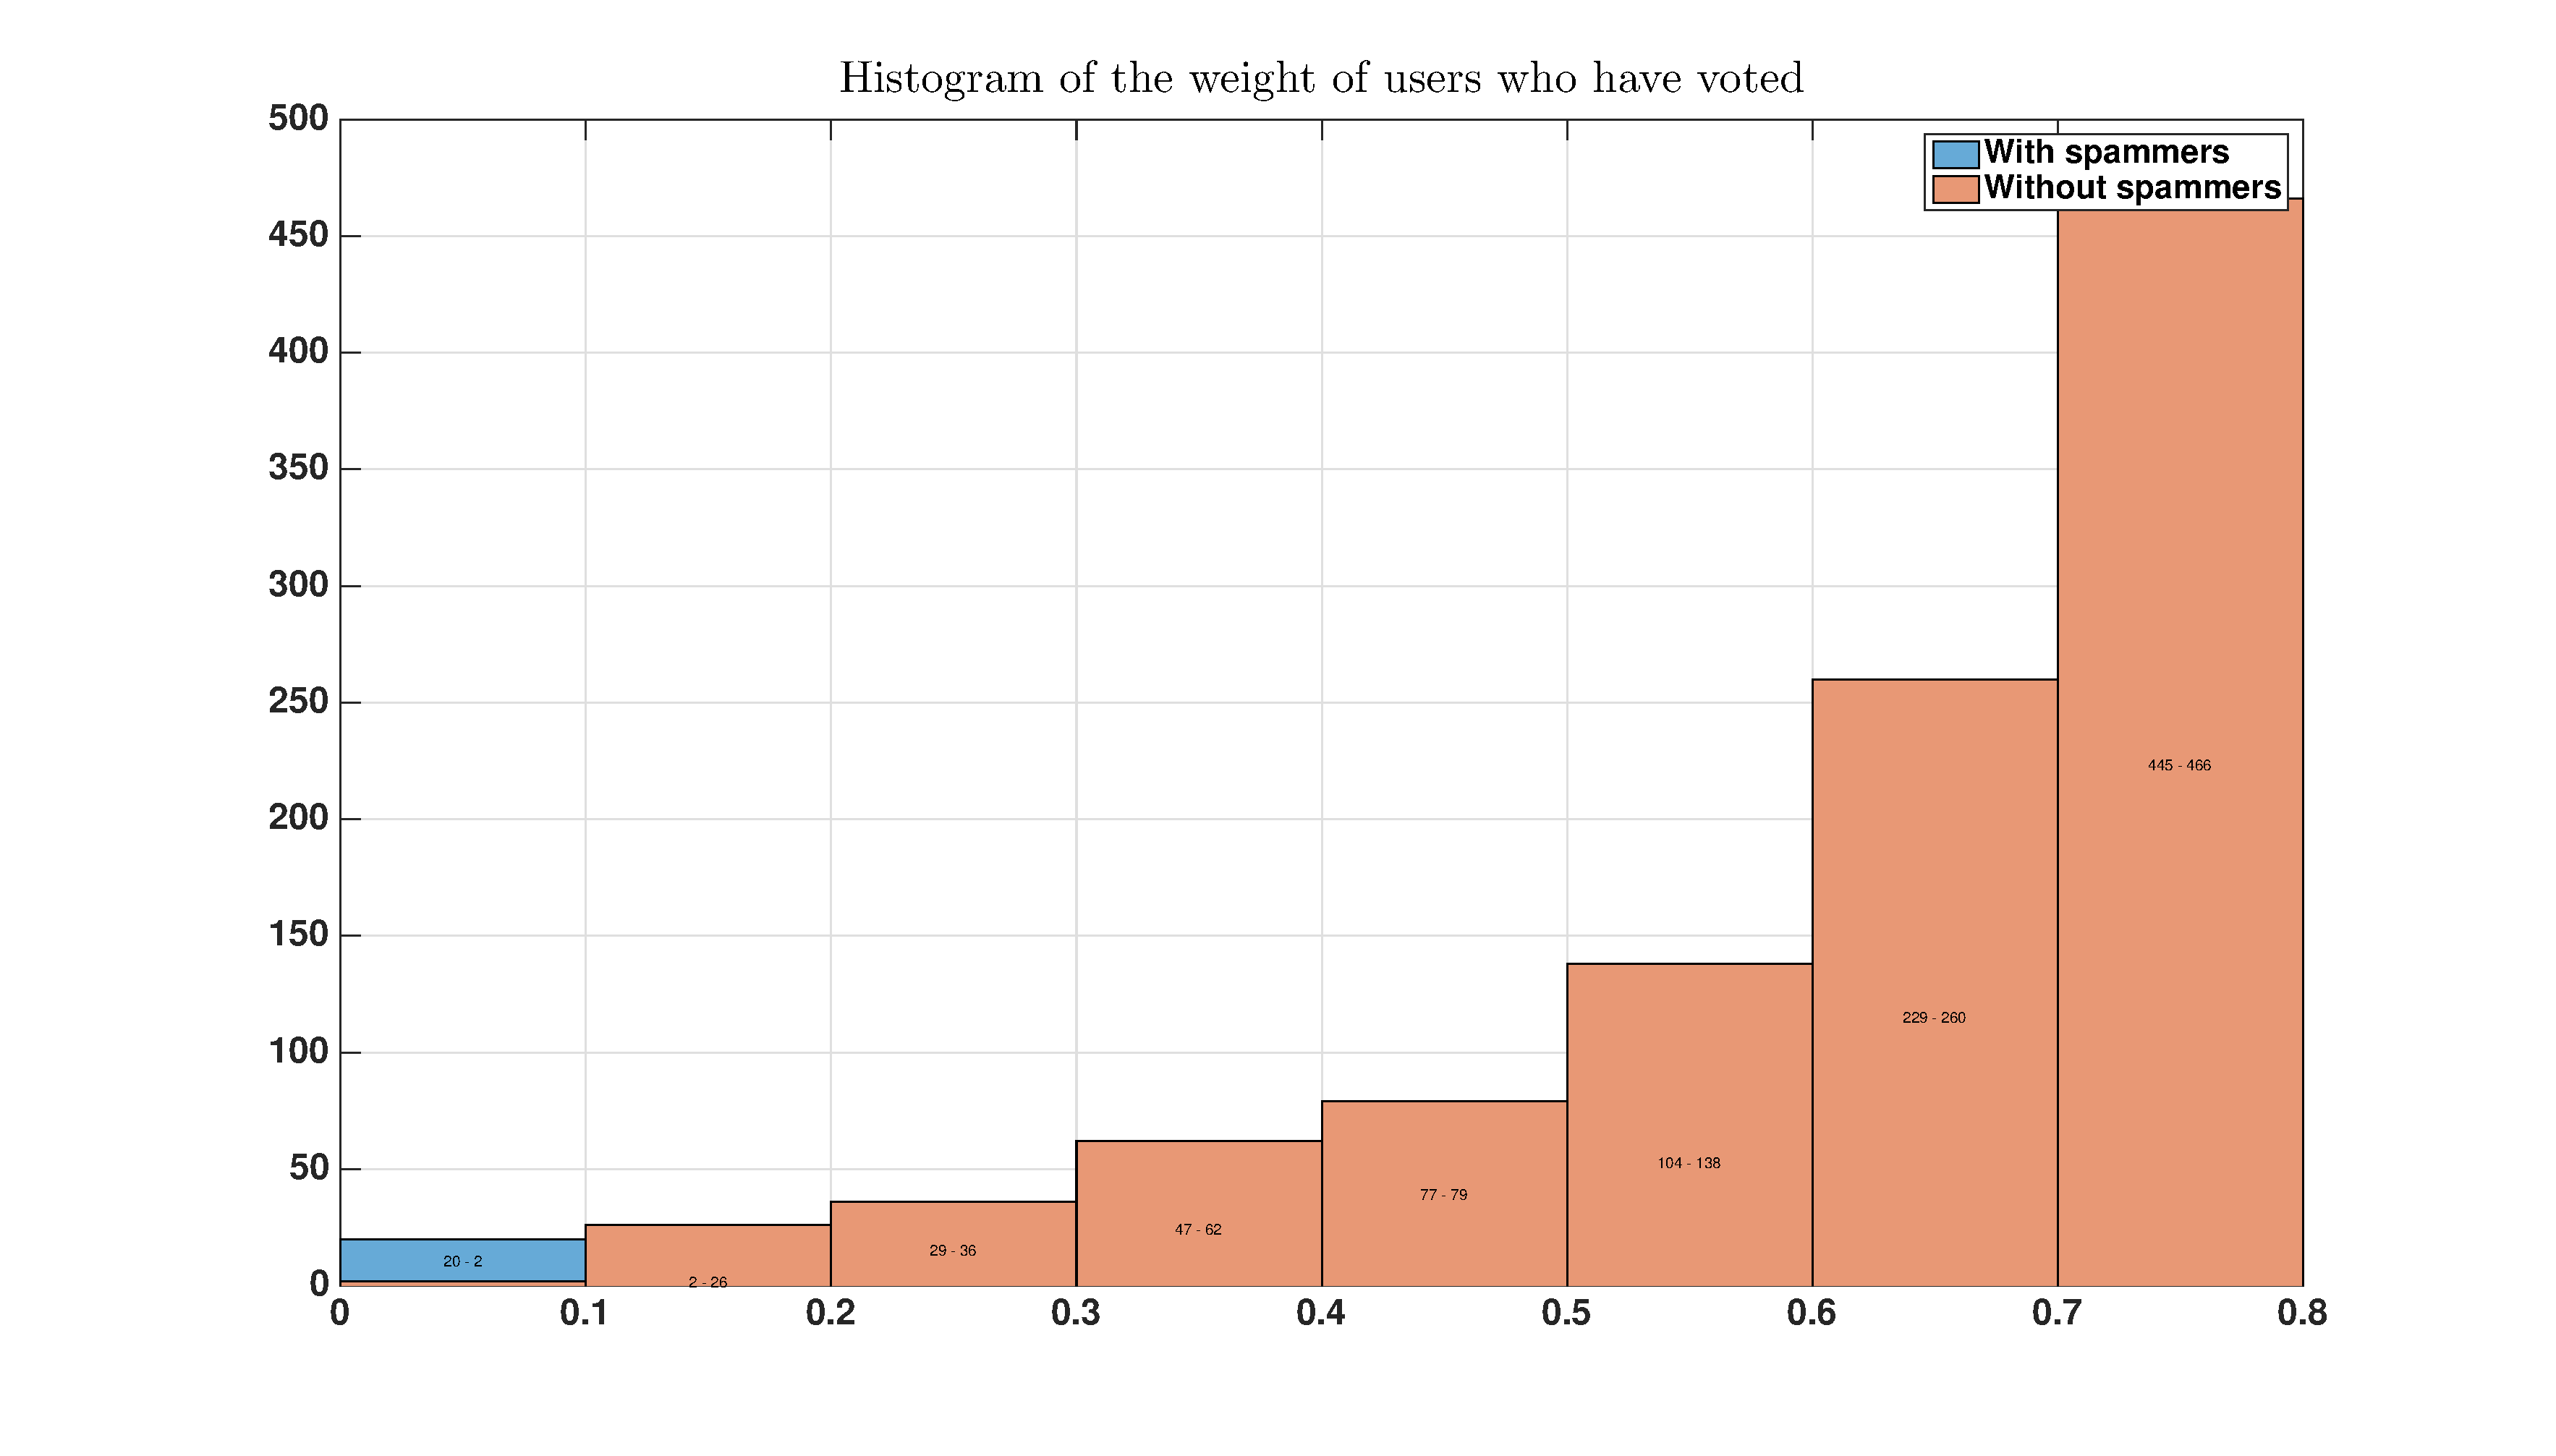
\includegraphics[width = \textwidth]{hotels/not_random_cheaters.eps}
\caption{\label{fig:hotel:not_random_cheaters} Distribution of weights after iterations with and without spammers}
\end{figure}

Here, spammers are perfectly spotted and their weight is quite low.\\

We now added to the original data set one spammer per hotel giving always 0 except for their own hotel, which they rated 5. The figure (\ref{fig:hotel:not_random_each_hotel}) illustrates the distribution of weights after iteration with and without spammers.

\begin{figure}[!h]
\centering
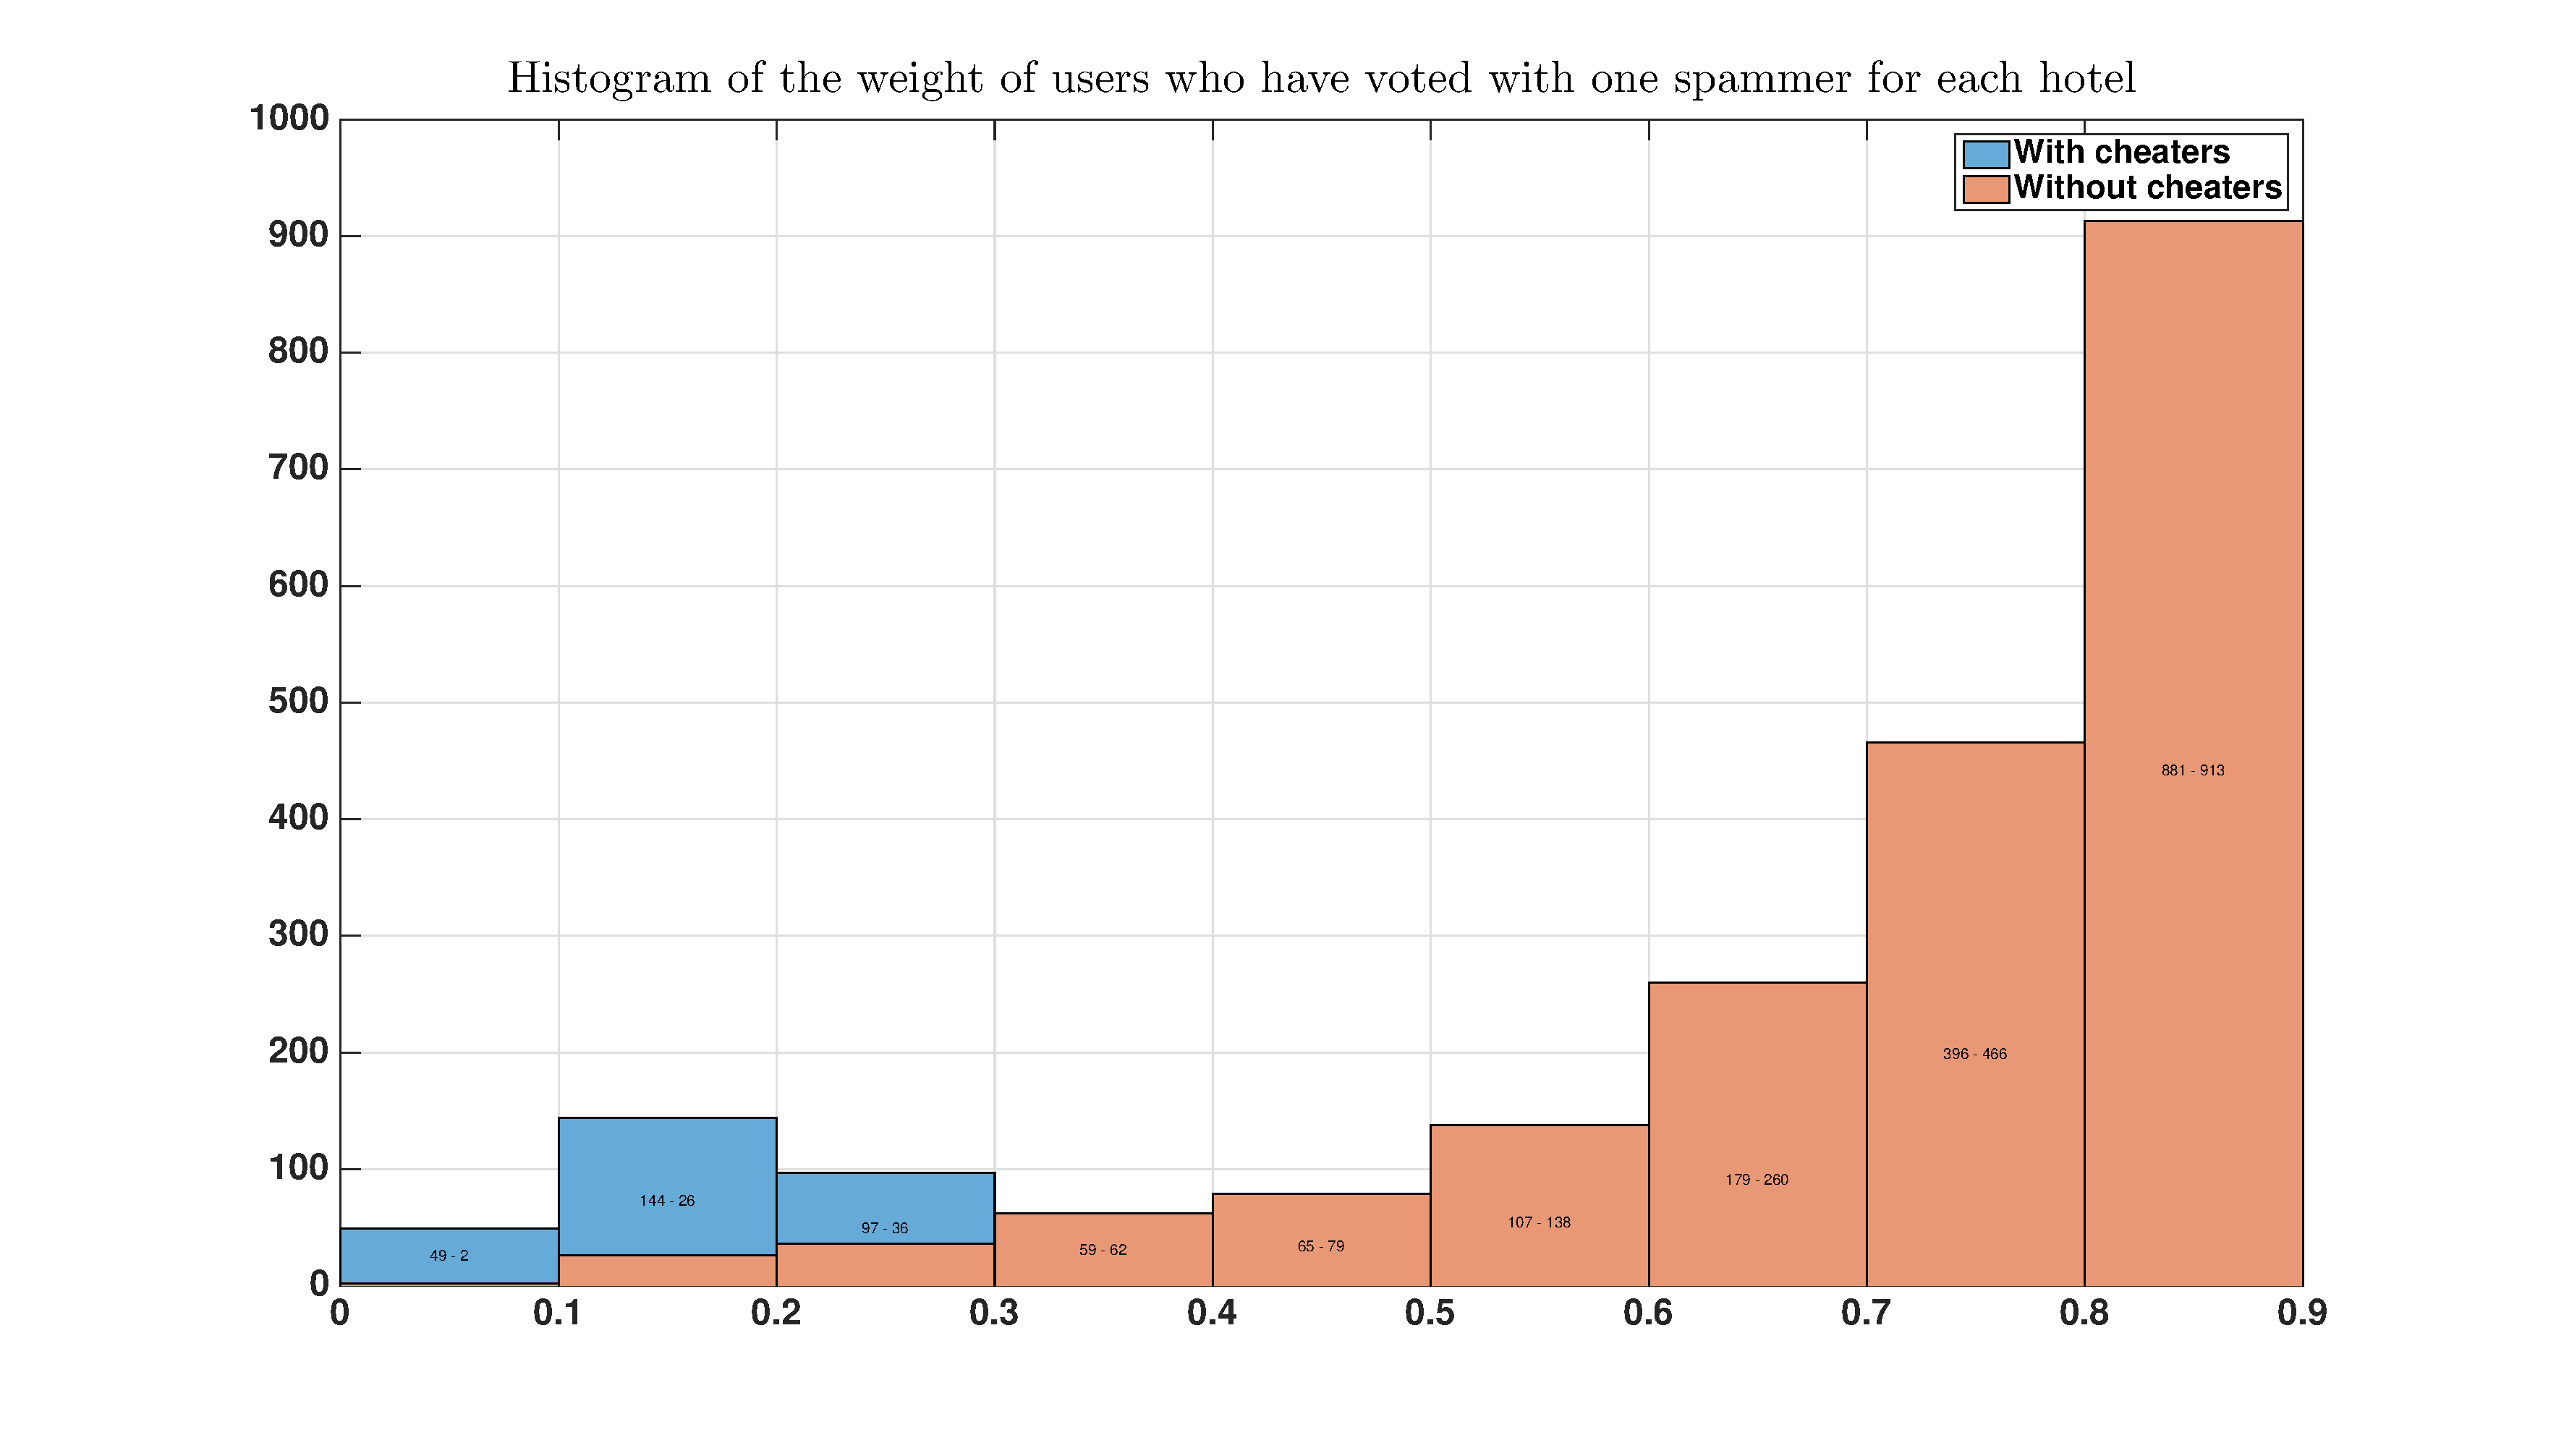
\includegraphics[width = \textwidth]{hotels/not_random_each_hotels.eps}
\caption{\label{fig:hotel:not_random_each_hotel} Distribution of weights after iterations with and without spammers}
\end{figure}

Here, spammers are perfectly spotted and their weight is quite low.

\FloatBarrier
\section{Conclusion}

\bibliographystyle{plain}
\bibliography{rapport/bib/biblio}
\nocite{*}


\end{document}